\documentclass[a4paper]{article}

\usepackage[english]{babel}
\usepackage[utf8]{inputenc}
\usepackage{amsmath}
\usepackage{graphicx}
\usepackage{caption}
\usepackage{subcaption}
\usepackage[colorinlistoftodos]{todonotes}

\title{Kernel Density Estimation And Hypothesis Testing on Persistence Diagrams}
\author{Mike Wu}

\begin{document}
\maketitle
\section{Kernel Density Exploration}
Strangely enough, the axis on the TDA website are flipped when compared to the ones generated using the same code provided by the tutorial. Most likely, this is an outdated tutorial. Or perhaps, I must manually flip the axis? More evidence of a possible typo: The rotated and bar plots look rather identical to the plots in the tutorial so it should be doing the same thing. Given that, why does the 1st order feature appear first? And why do so many additional 0th order features appear far later? Are these noisy perturbations? 

To peek deeper into what KDE does, let's try to plot the 3D topology of the smoothed gaussian curves.  First thing I notice is that things are extremely smoothed and that there exists only 1 obvious local maxima. If that is true than the KDE diagram makes sense since a 0th homology feature is found first (the tall peak) and then the 1st homology feature is found (the rest of the smooth circle). The residual 0th homologies, like the bands describe, are due to small bumps on the surface, i.e. noise perturbations. (Does this make sense?). \textbf{Observation 0: } The larger the object, i.e. radius of larger size, the smaller the gaussian peaks overlap, an the less prominent the overlaps. A circle of radius 10 will probably have many more small short-lived 0th homology features and a less prominent 1st homology feature than a circle of radius 1 (But when I ran it, the two actually look very similar, perhaps we can discuss it more). 

\begin{figure}[htp!]
\centering
\begin{subfigure}{.5\textwidth}
  \centering
  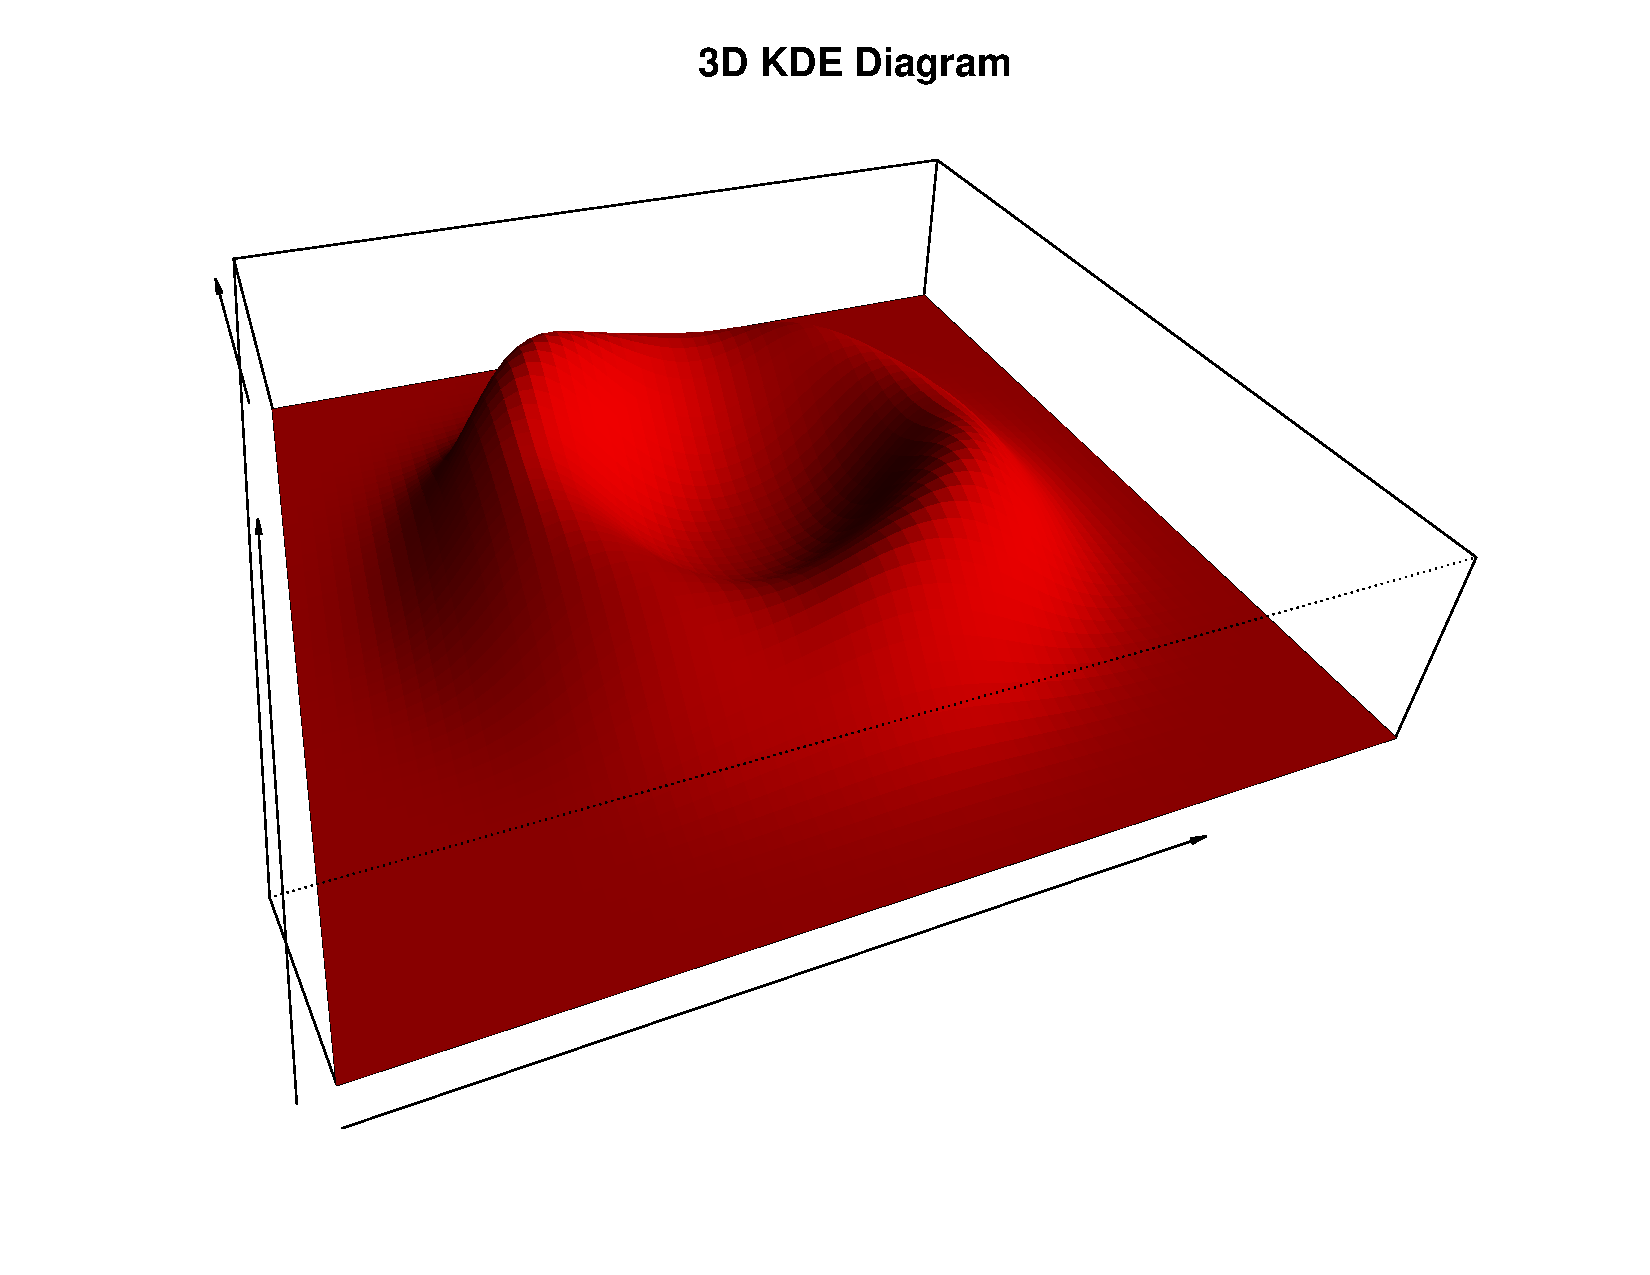
\includegraphics[width=\linewidth]{topograph}
\end{subfigure}%
\begin{subfigure}{.5\textwidth}
  \centering
  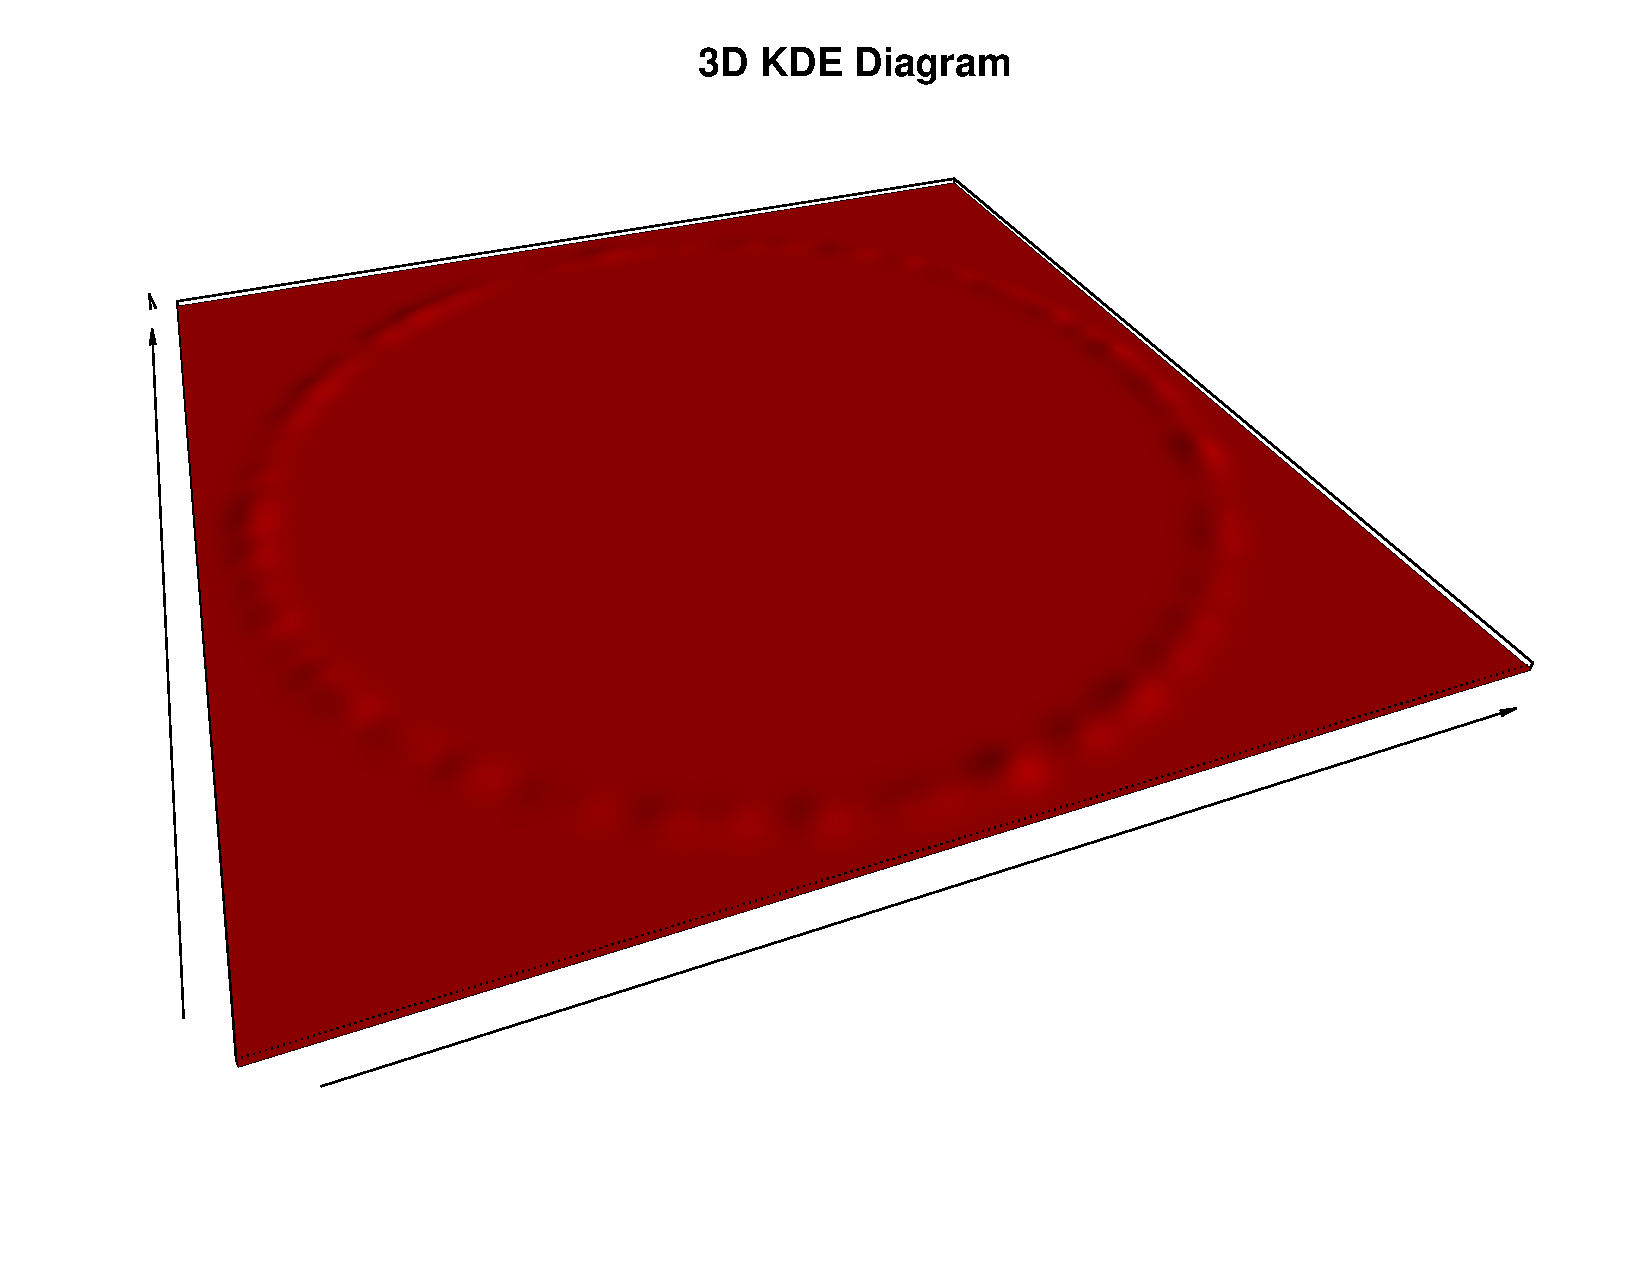
\includegraphics[width=\linewidth]{topograph2}
\end{subfigure}
\caption{3D graph of KDE for a uniform circle of radius (left) 1, (right) 10. }
\end{figure}

The algorithm has been reformatted to fit the TDA guide as well as add an additional confidence band (new Github commit). The objects above the band indicate those are statistically differentiable from noise. 

\begin{figure}[htp!]
\centering
\begin{subfigure}{.5\textwidth}
  \centering
  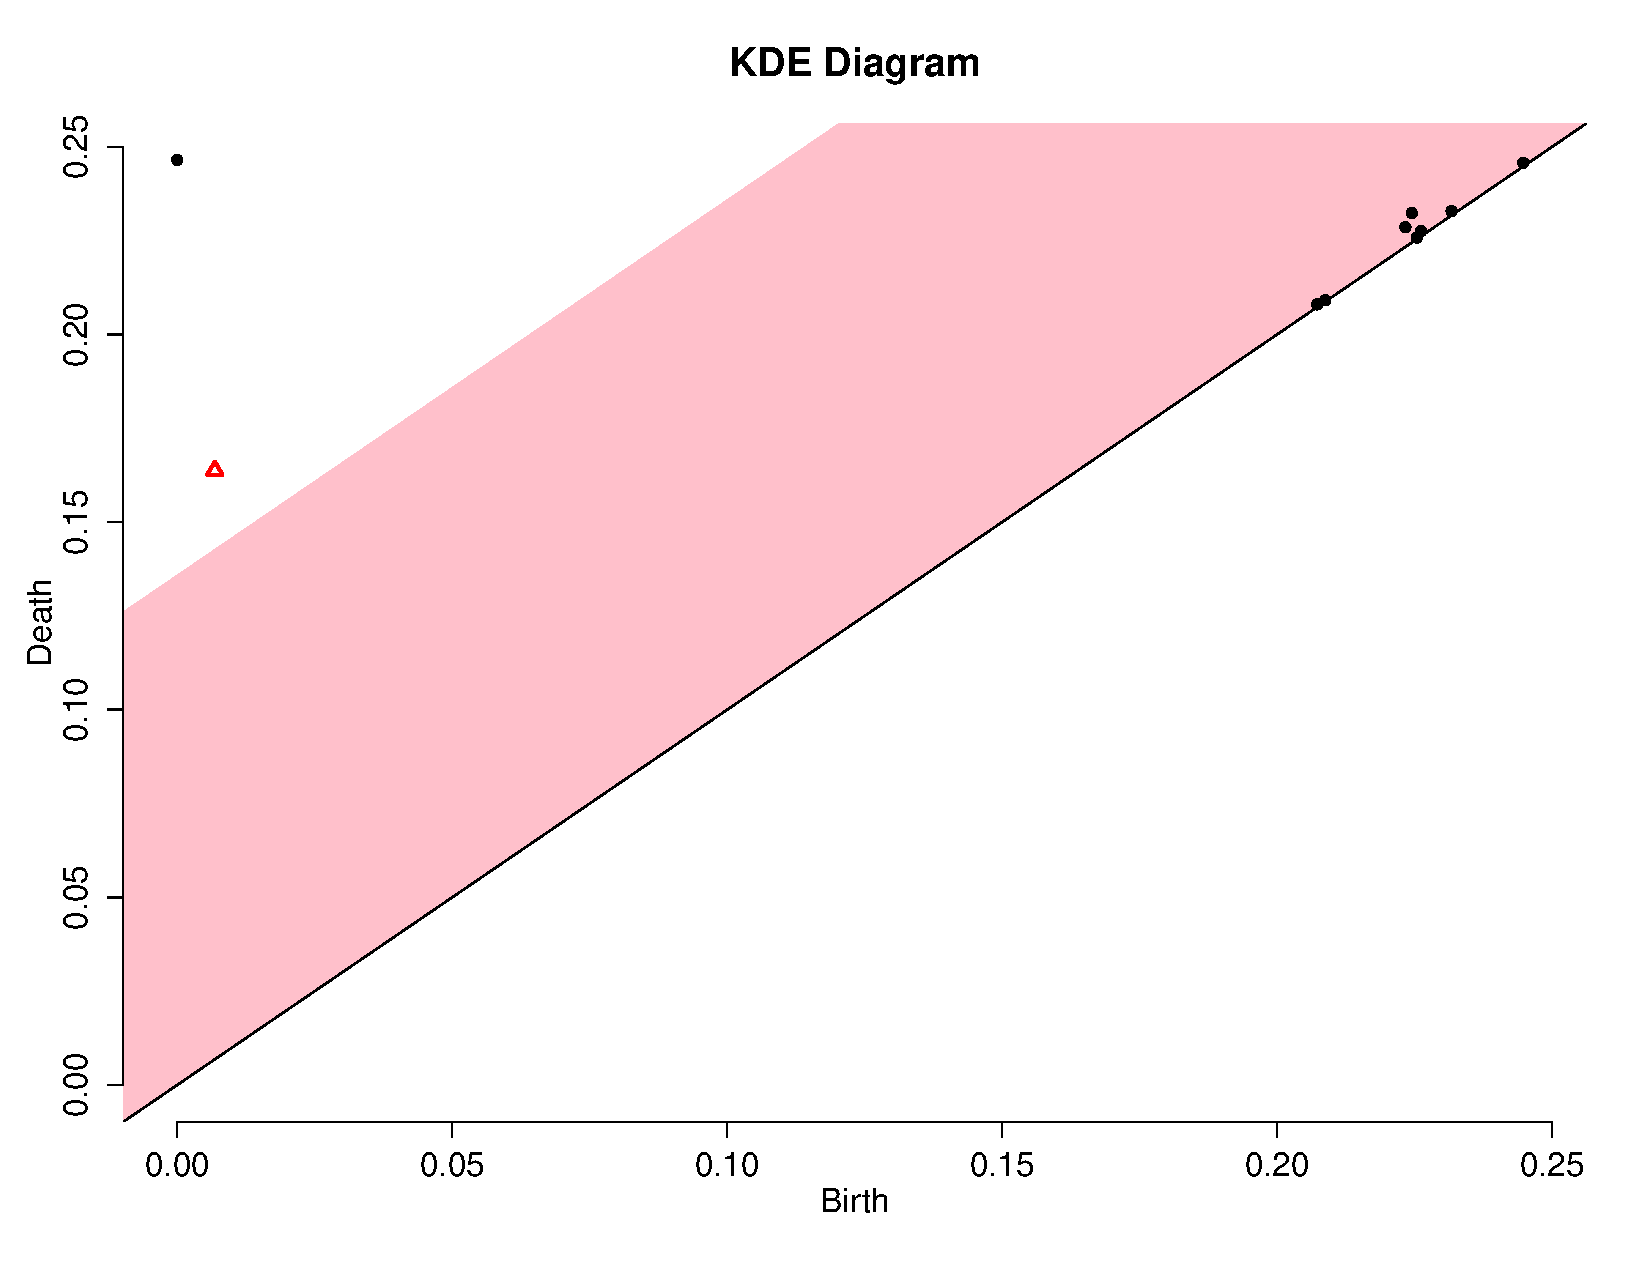
\includegraphics[width=\linewidth]{KDEweek2}
\end{subfigure}%
\begin{subfigure}{.5\textwidth}
  \centering
  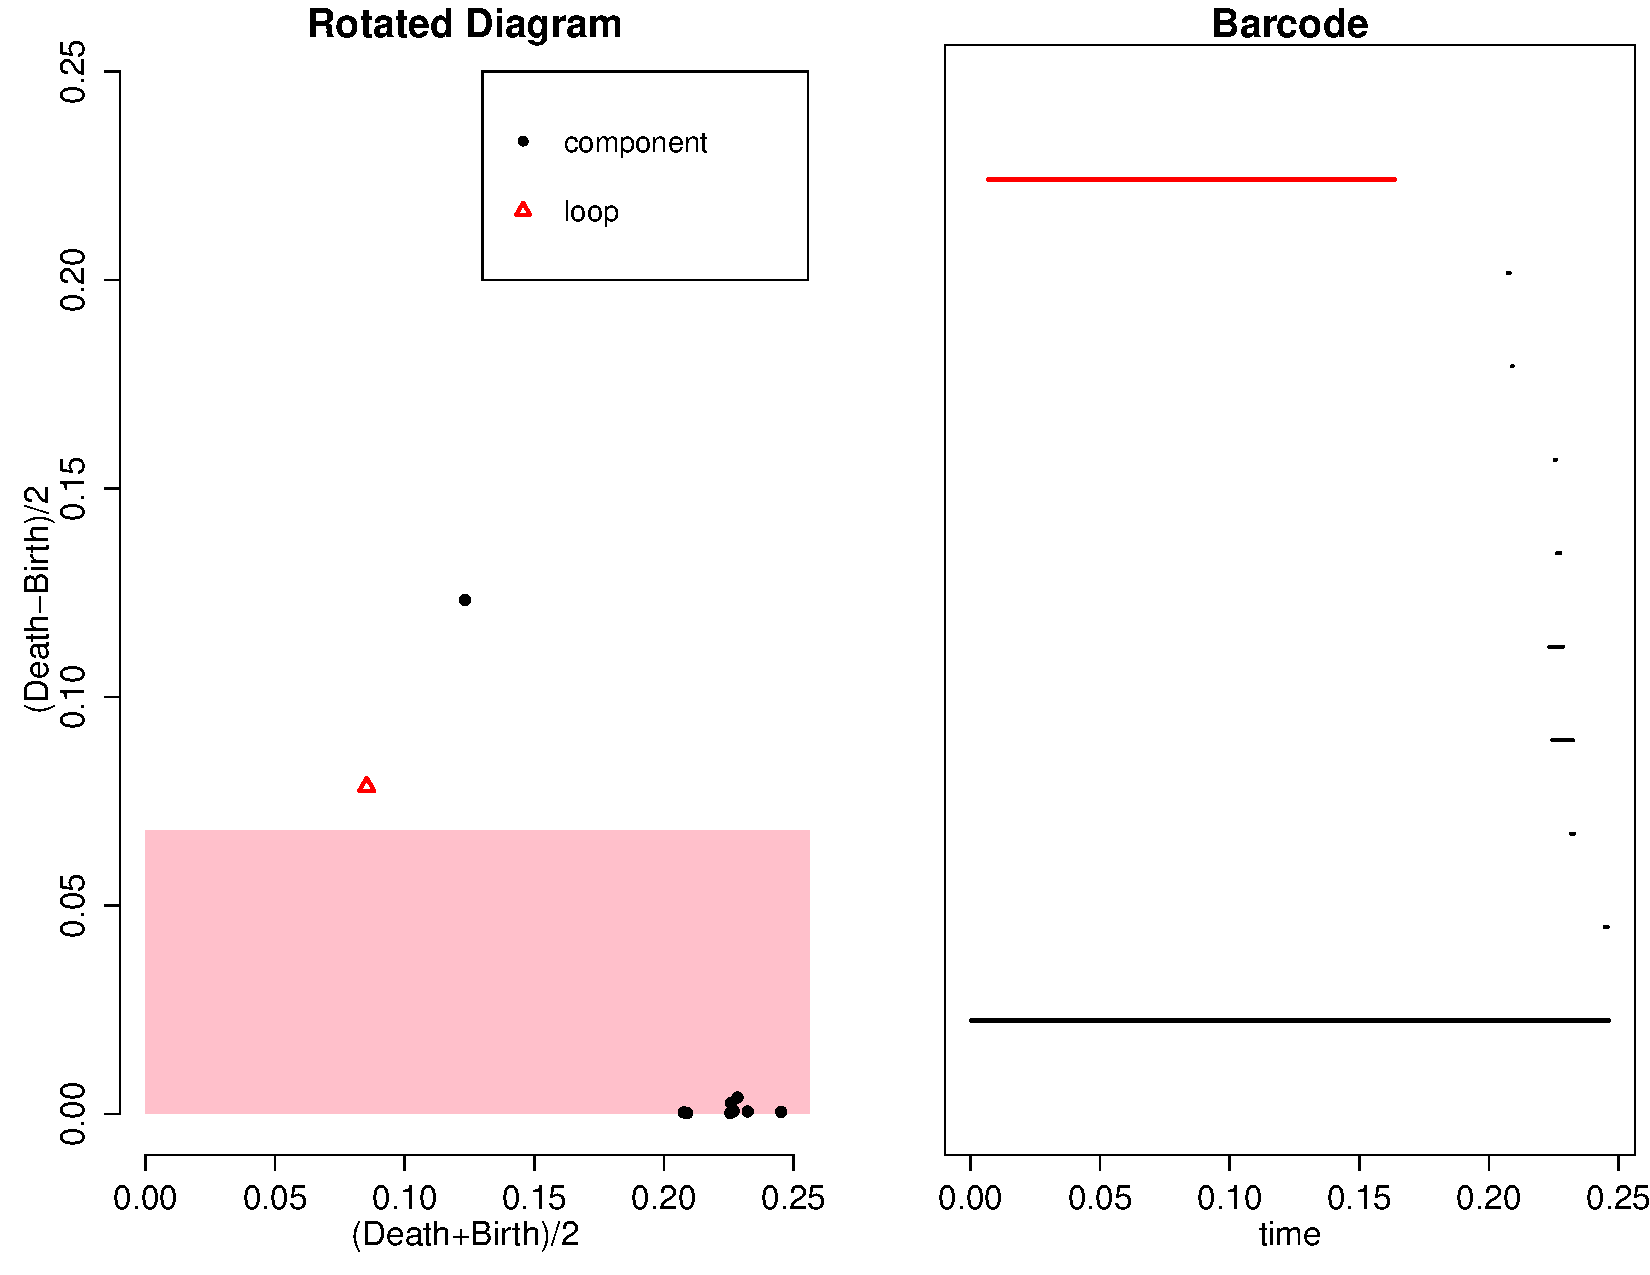
\includegraphics[width=\linewidth]{rotatedKDE}
\end{subfigure}
\caption{(Left) Regular KDE Diagram from a uniform circle with a band representing a significance level. (Middle) Rotated KDE Diagram. (Right) Bar Diagram.}
\end{figure}

We can also explore the effect of different parameters on the KDE system. \textbf{Observation 1:} the more samples generated from each uniform circle, the smaller the area imputed to noise. This makes sense since we are more confident that a circle exists, and attribute less of the space to random objects. \textbf{Observation 2:} $h$ is the smoothing factor, and the higher the smoothing factor, the more confident we are that less area is attributed to noise. This also makes sense, since increasing $h$ is almost equivalent to applying a stronger gaussian smoothing filter, whose primary role is to nullify noise. Notice in this case we didn't lose much resolution because there is such a clear defined object. In more difficult cases, increasing $h$ too much probably loses resolution. \textbf{Observation 3:} The grid for which KDE is built on affects the confidence level on noise. Very small grid sizes have lower confidence intervals, and as you increase the grid sizes the noisy areas increase, probably suggesting that we are losing resolution. Strangely enough as you increase the grid even more, to remarkably high levels, the noisy areas diminish fast with seemingly no loss in homological objects. I am not sure why this is happening?

\begin{figure}[htp!]
\centering
\begin{subfigure}{.5\textwidth}
  \centering
  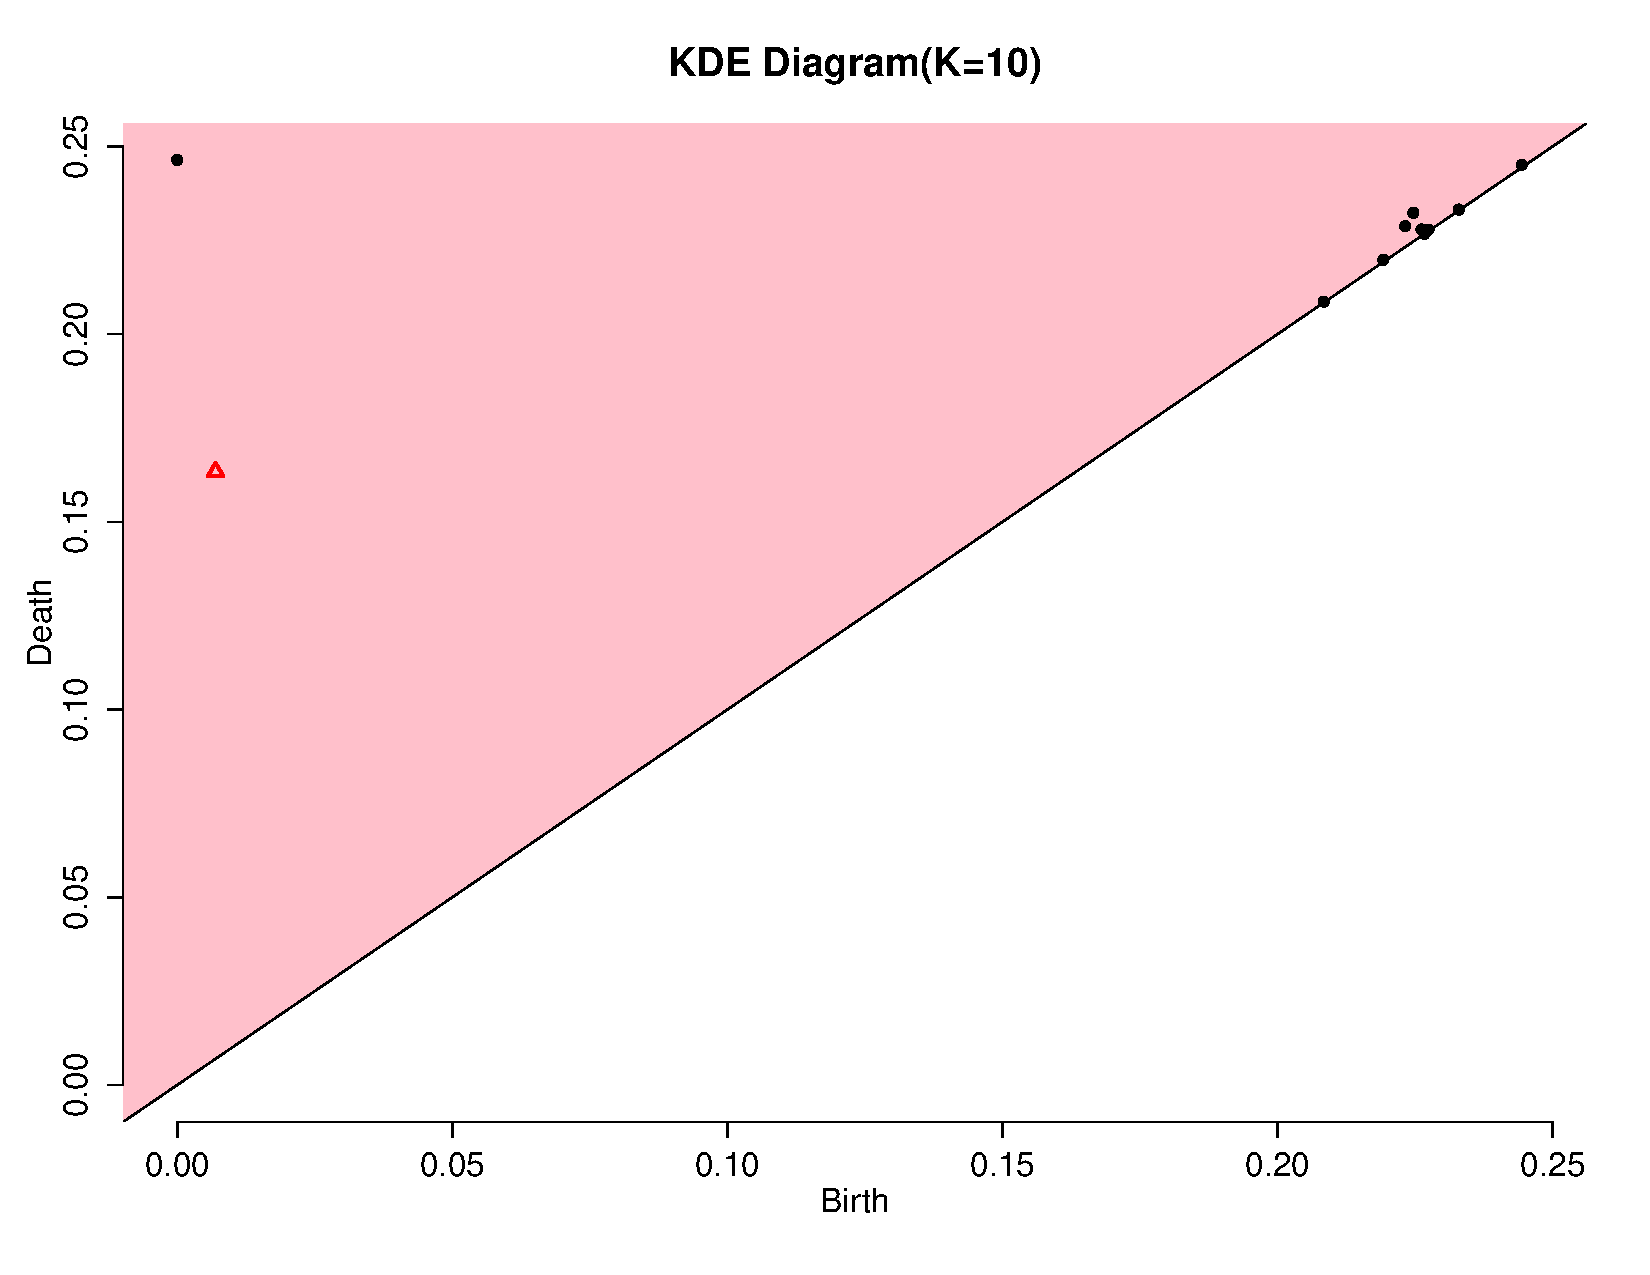
\includegraphics[width=\linewidth]{KDE-K10}
\end{subfigure}%
\begin{subfigure}{.5\textwidth}
  \centering
  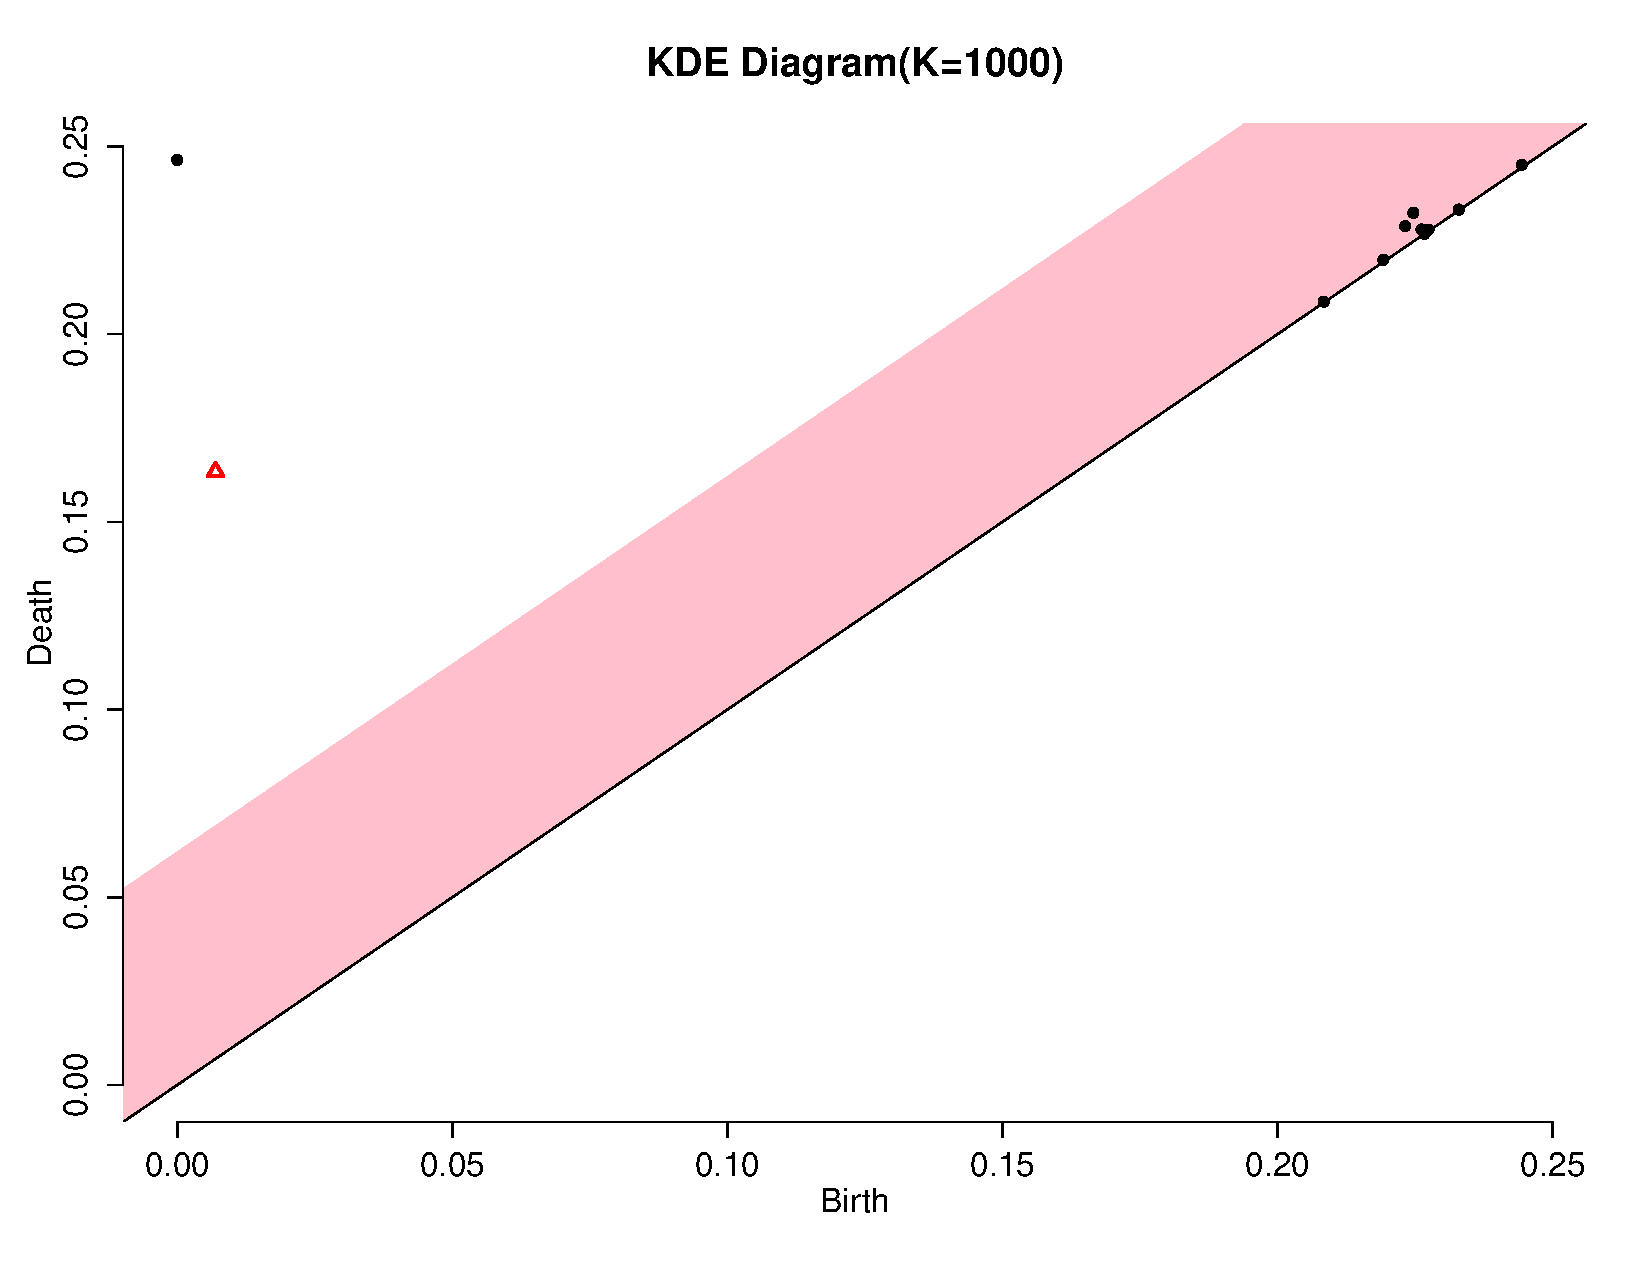
\includegraphics[width=\linewidth]{KDE-k1000}
\end{subfigure}
\caption{(Left) KDE of uniform circle with 10 points. (Right) KDE of uniform circle with 1000 points.}
\end{figure}

\begin{figure}[htb!]
\centering
\begin{subfigure}{.32\textwidth}
  \centering
  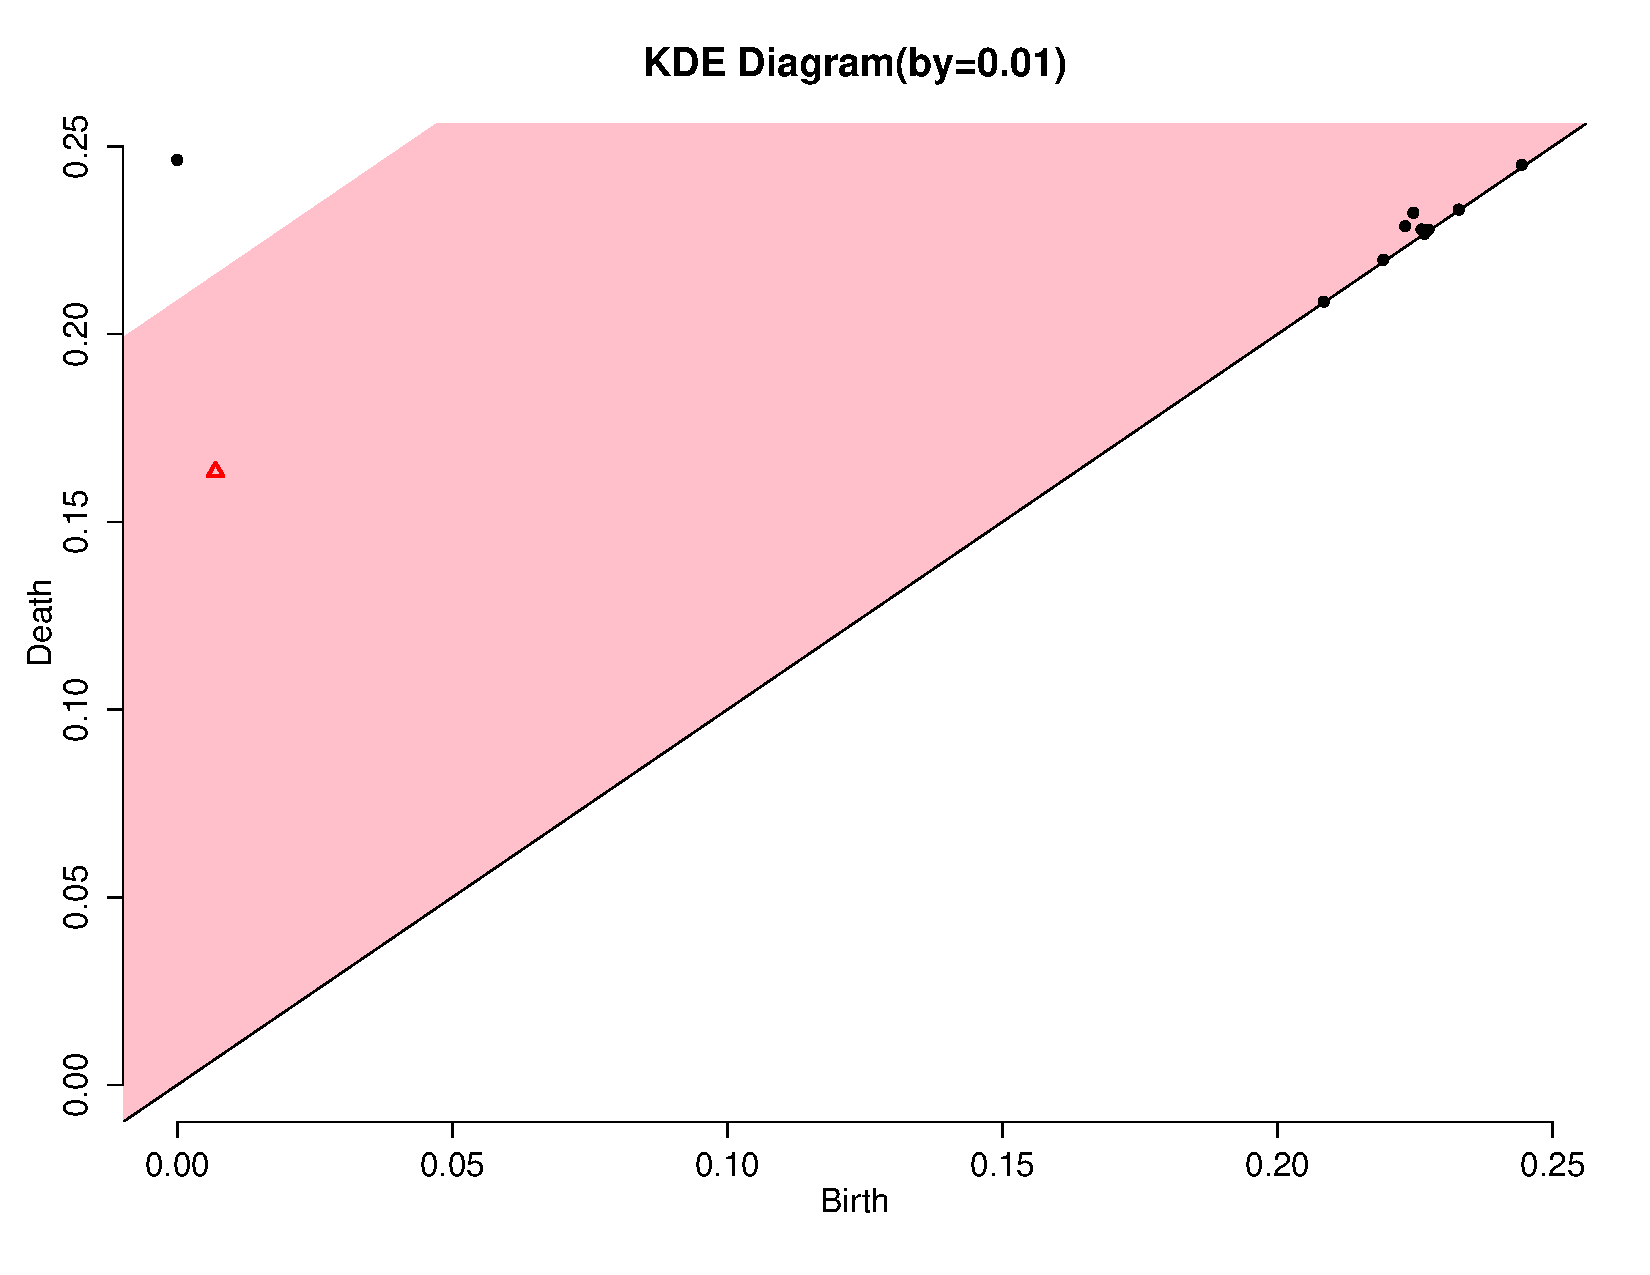
\includegraphics[width=\linewidth]{KDE-by0_01}
\end{subfigure}%
\begin{subfigure}{.32\textwidth}
  \centering
  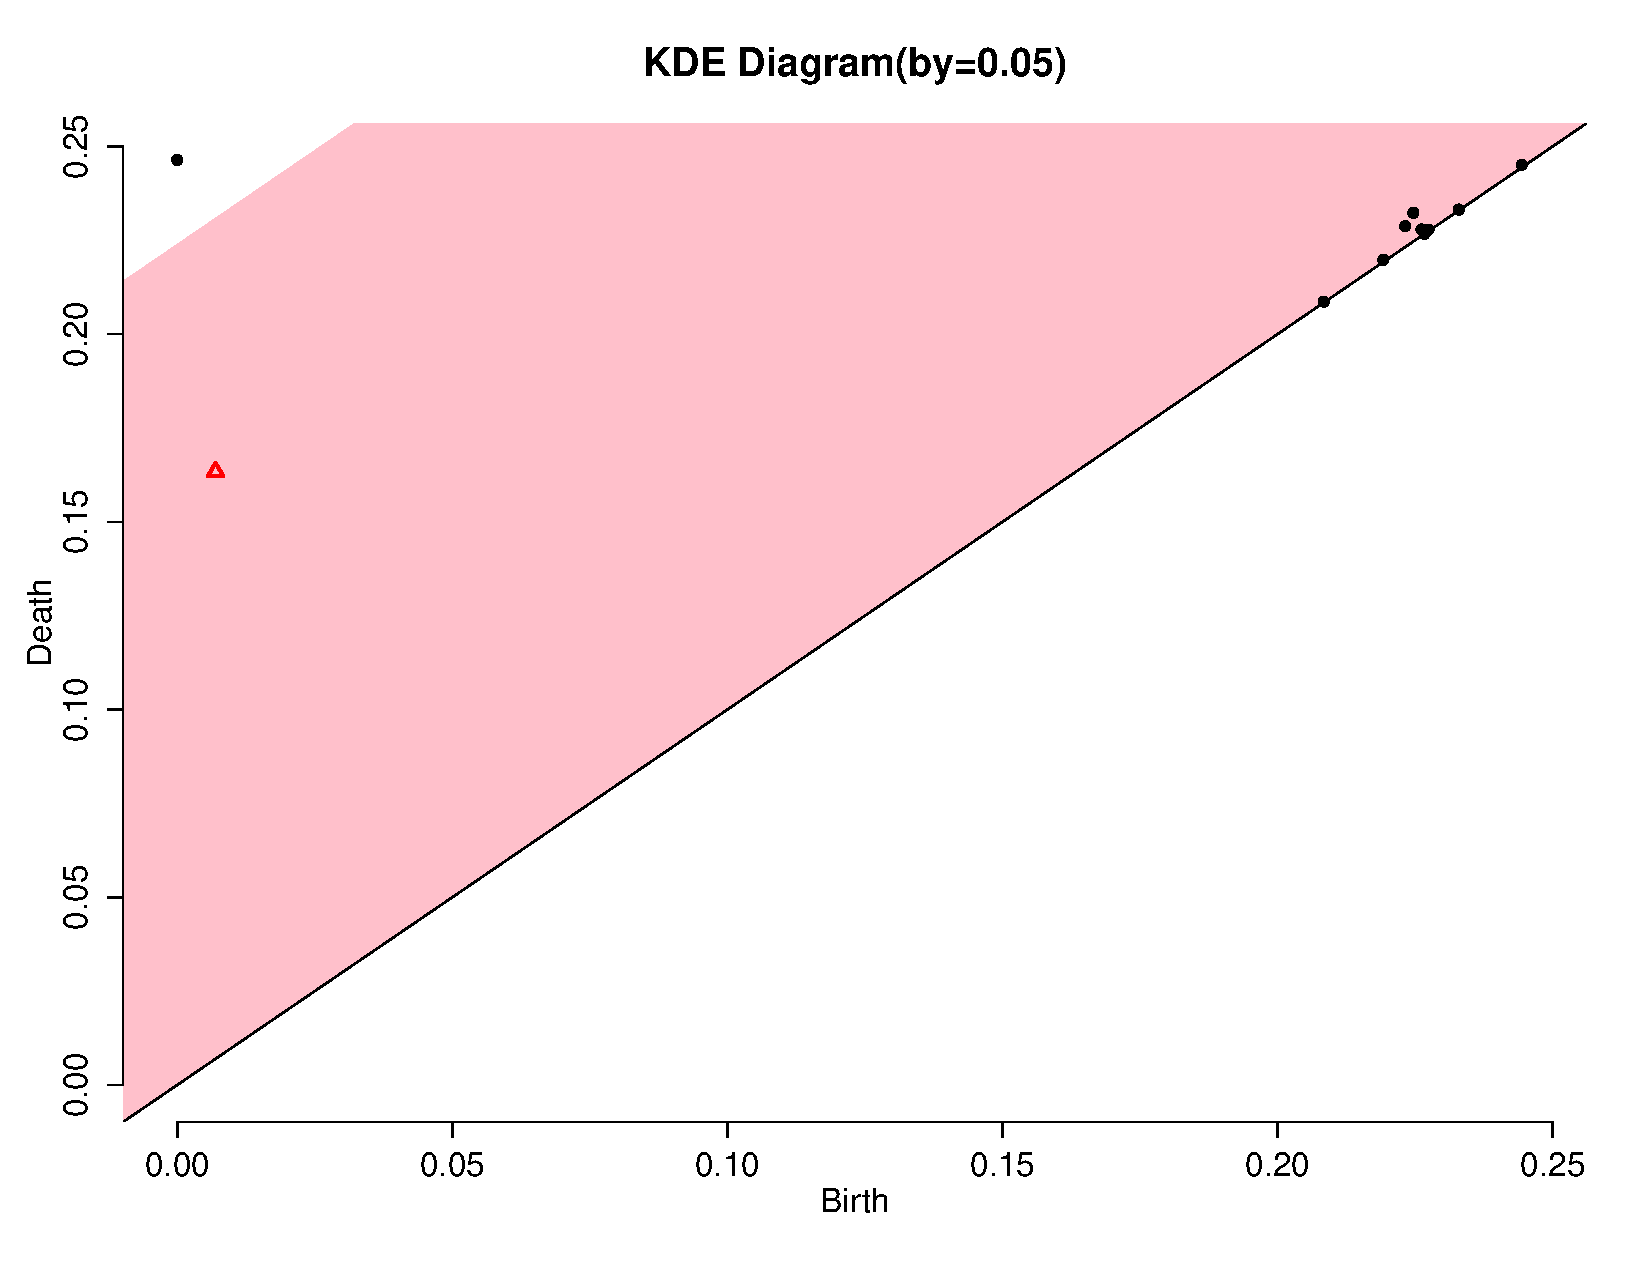
\includegraphics[width=\linewidth]{KDE-by0_05}
\end{subfigure}
\begin{subfigure}{.32\textwidth}
  \centering
  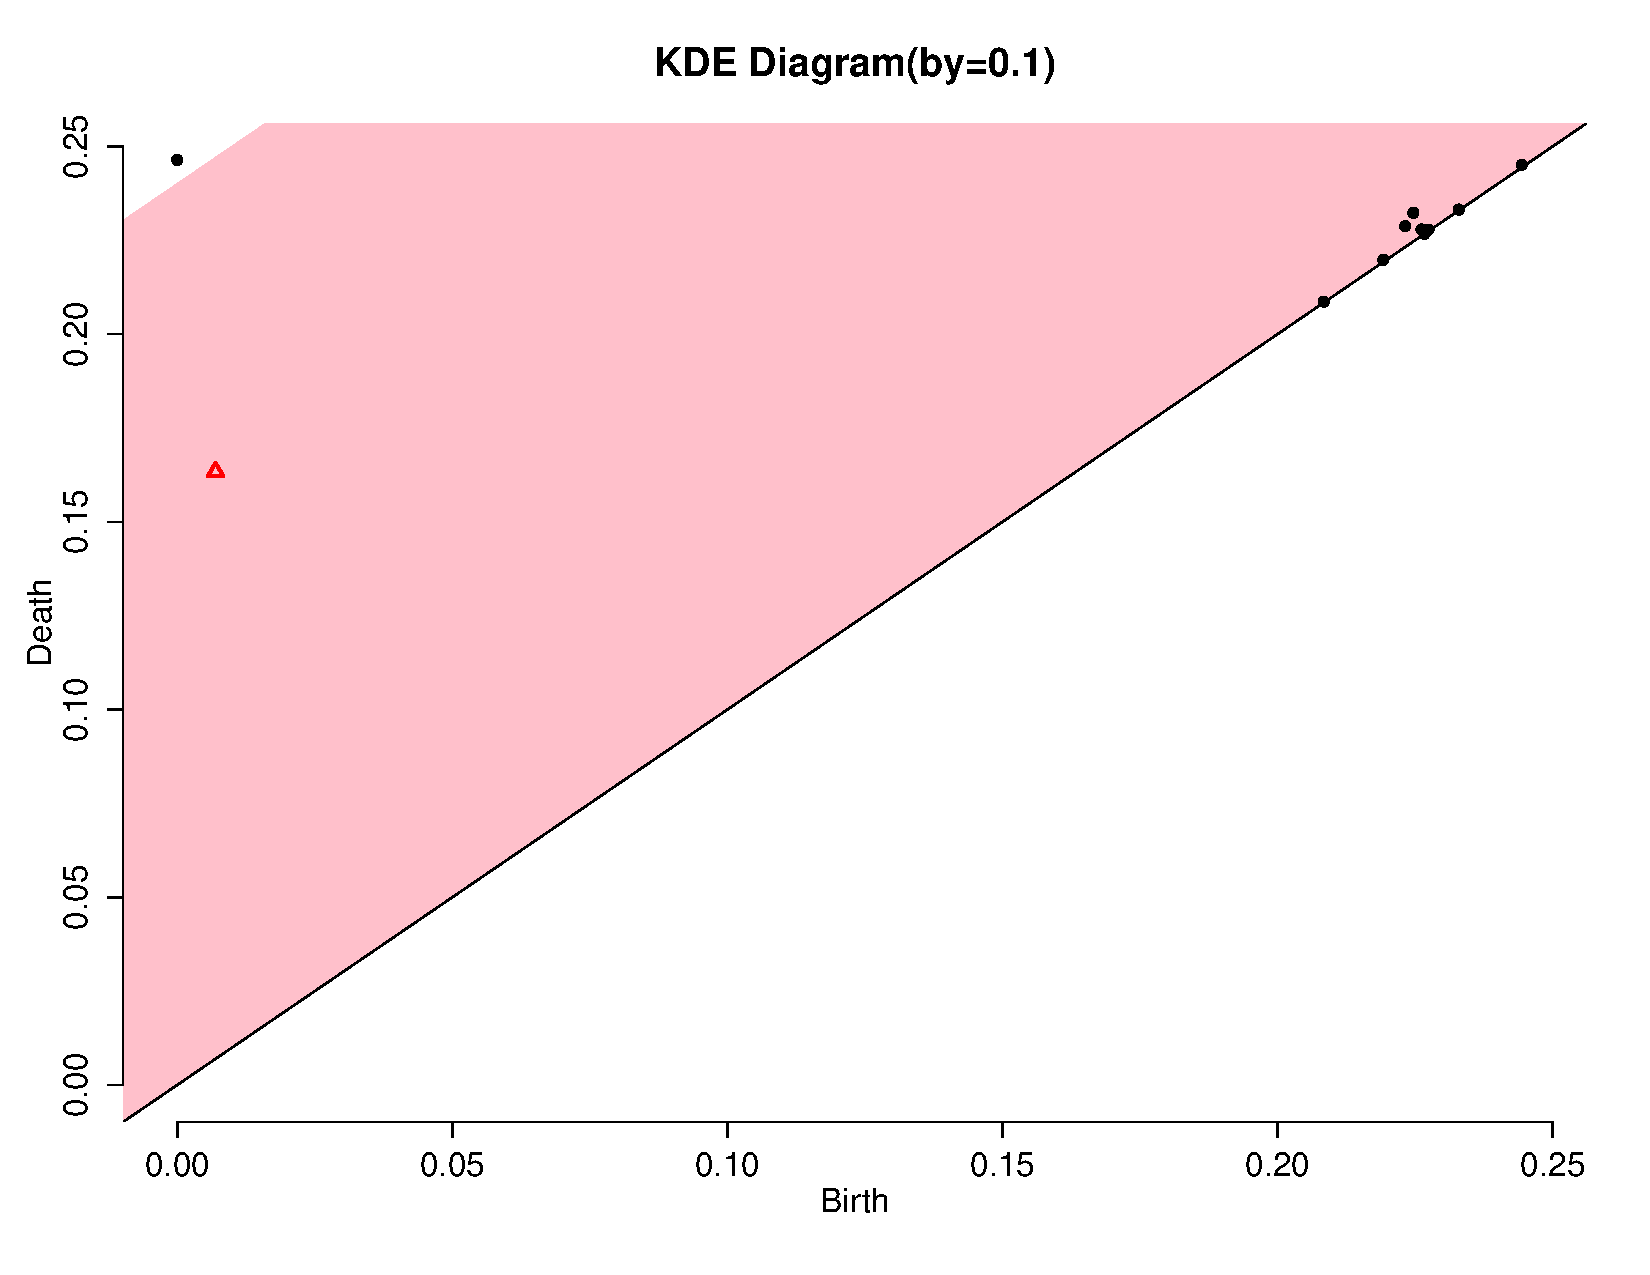
\includegraphics[width=\linewidth]{KDE-by0_1}
\end{subfigure}
\begin{subfigure}{.32\textwidth}
  \centering
  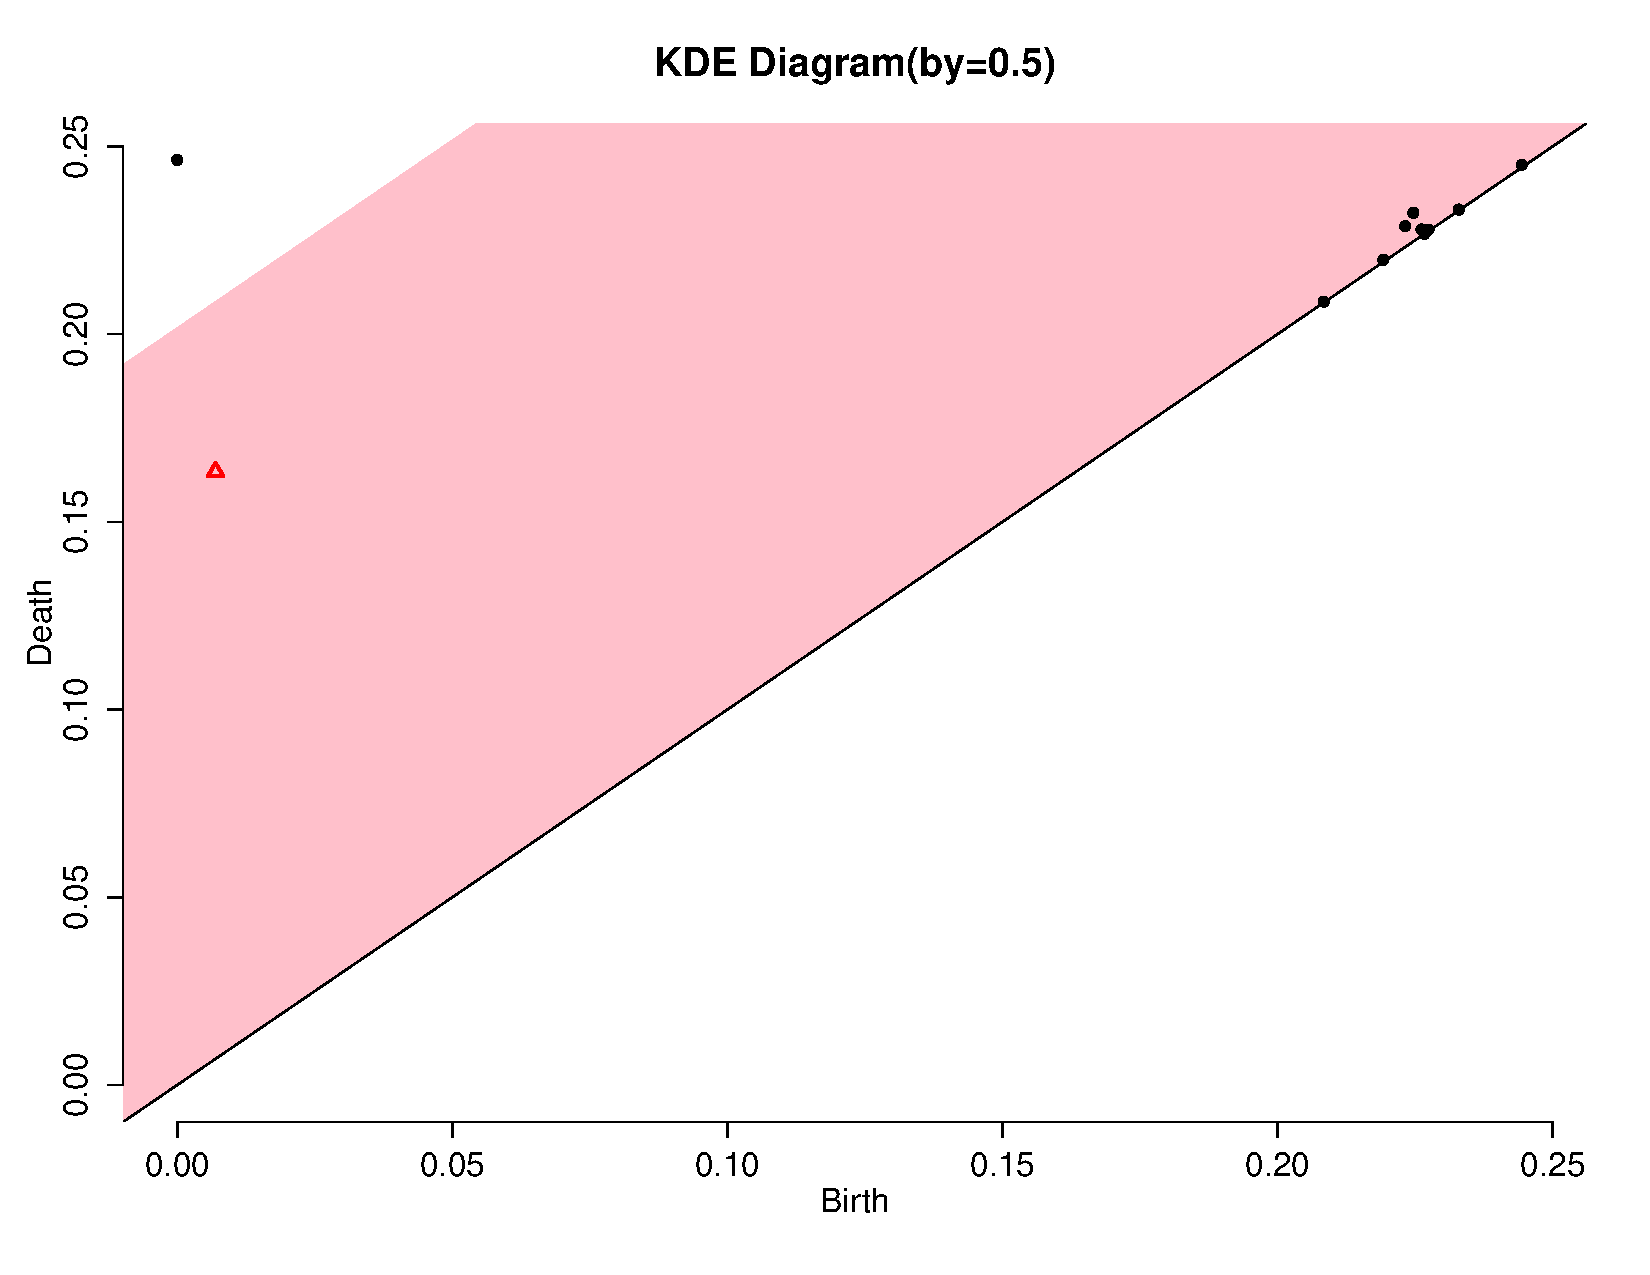
\includegraphics[width=\linewidth]{KDE-by0_5}
\end{subfigure}
\begin{subfigure}{.32\textwidth}
  \centering
  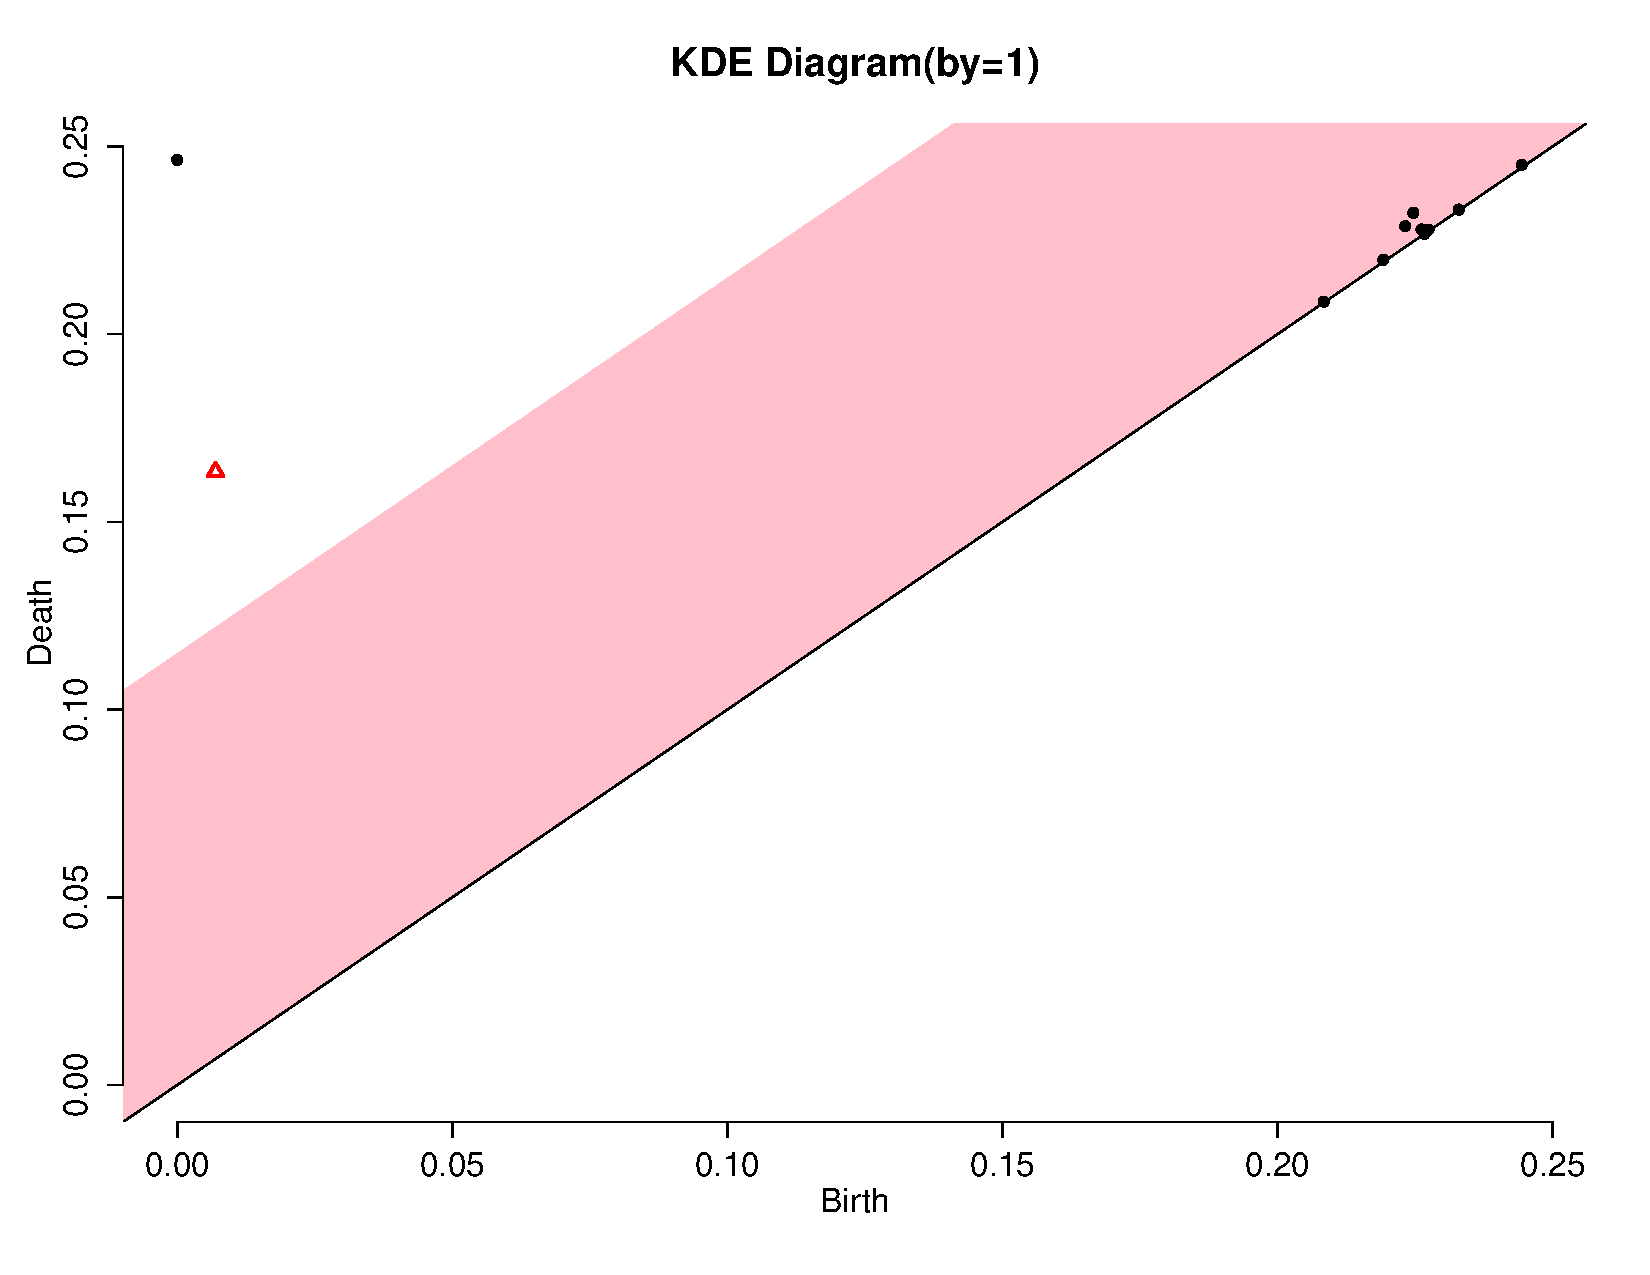
\includegraphics[width=\linewidth]{KDE-by1}
\end{subfigure}
\caption{Persistence diagrams of a uniform circle with different grid step sizes. The amount of noise coverage is seemingly parabolic with step size.}
\end{figure}

\section{Noisy Kernel Densities}
Last week, I investigated the Rips Complex and noticed that it does not handle noisy data very well. Because it gives each point equal weight, noise easily clouds any true structure. Intuitively, kernel density should be more robust since noise would be equivalent to small maxima. 

\subsection{Perturbing Points on the Circle}
Each of the $K$ points sampled from the uniform circle is shifted a little by a small Gaussian noise. Let's go with something extreme and sample from $\sim N(0, 1)$ with a circle of radius $5$. Generally, it seems like this definitely does handle noise better, but adding some noise does produce a lot of short-lived 1st  homology features and long-lived 0th homology features, which may distract from the true structure. This may have important consequences when conducting hypothesis tests between persistence diagrams since as figure 5 shows, the persistence diagram of noisy data is also noisy.

\begin{figure}[htp!]
\centering
\begin{subfigure}{.32\textwidth}
  \centering
  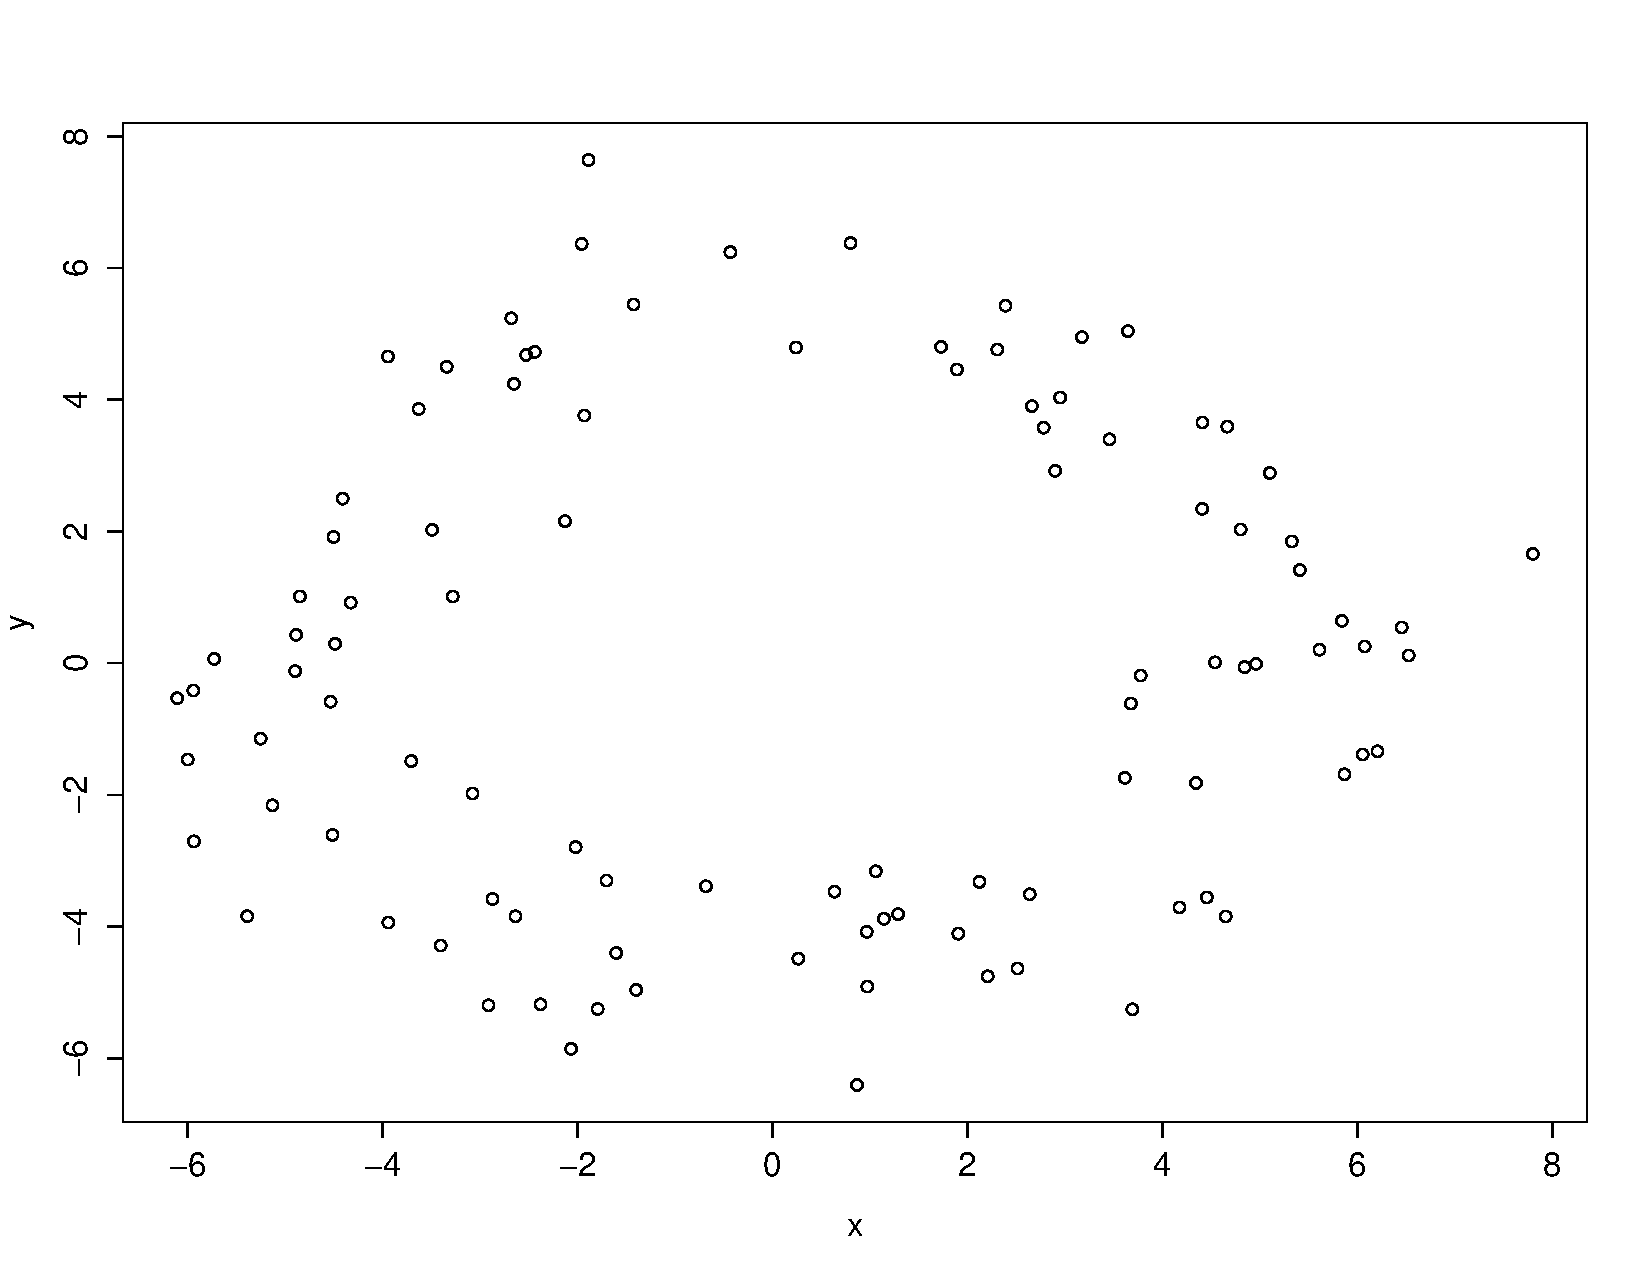
\includegraphics[width=\linewidth]{noisecircle1}
\end{subfigure}%
\begin{subfigure}{.32\textwidth}
  \centering
  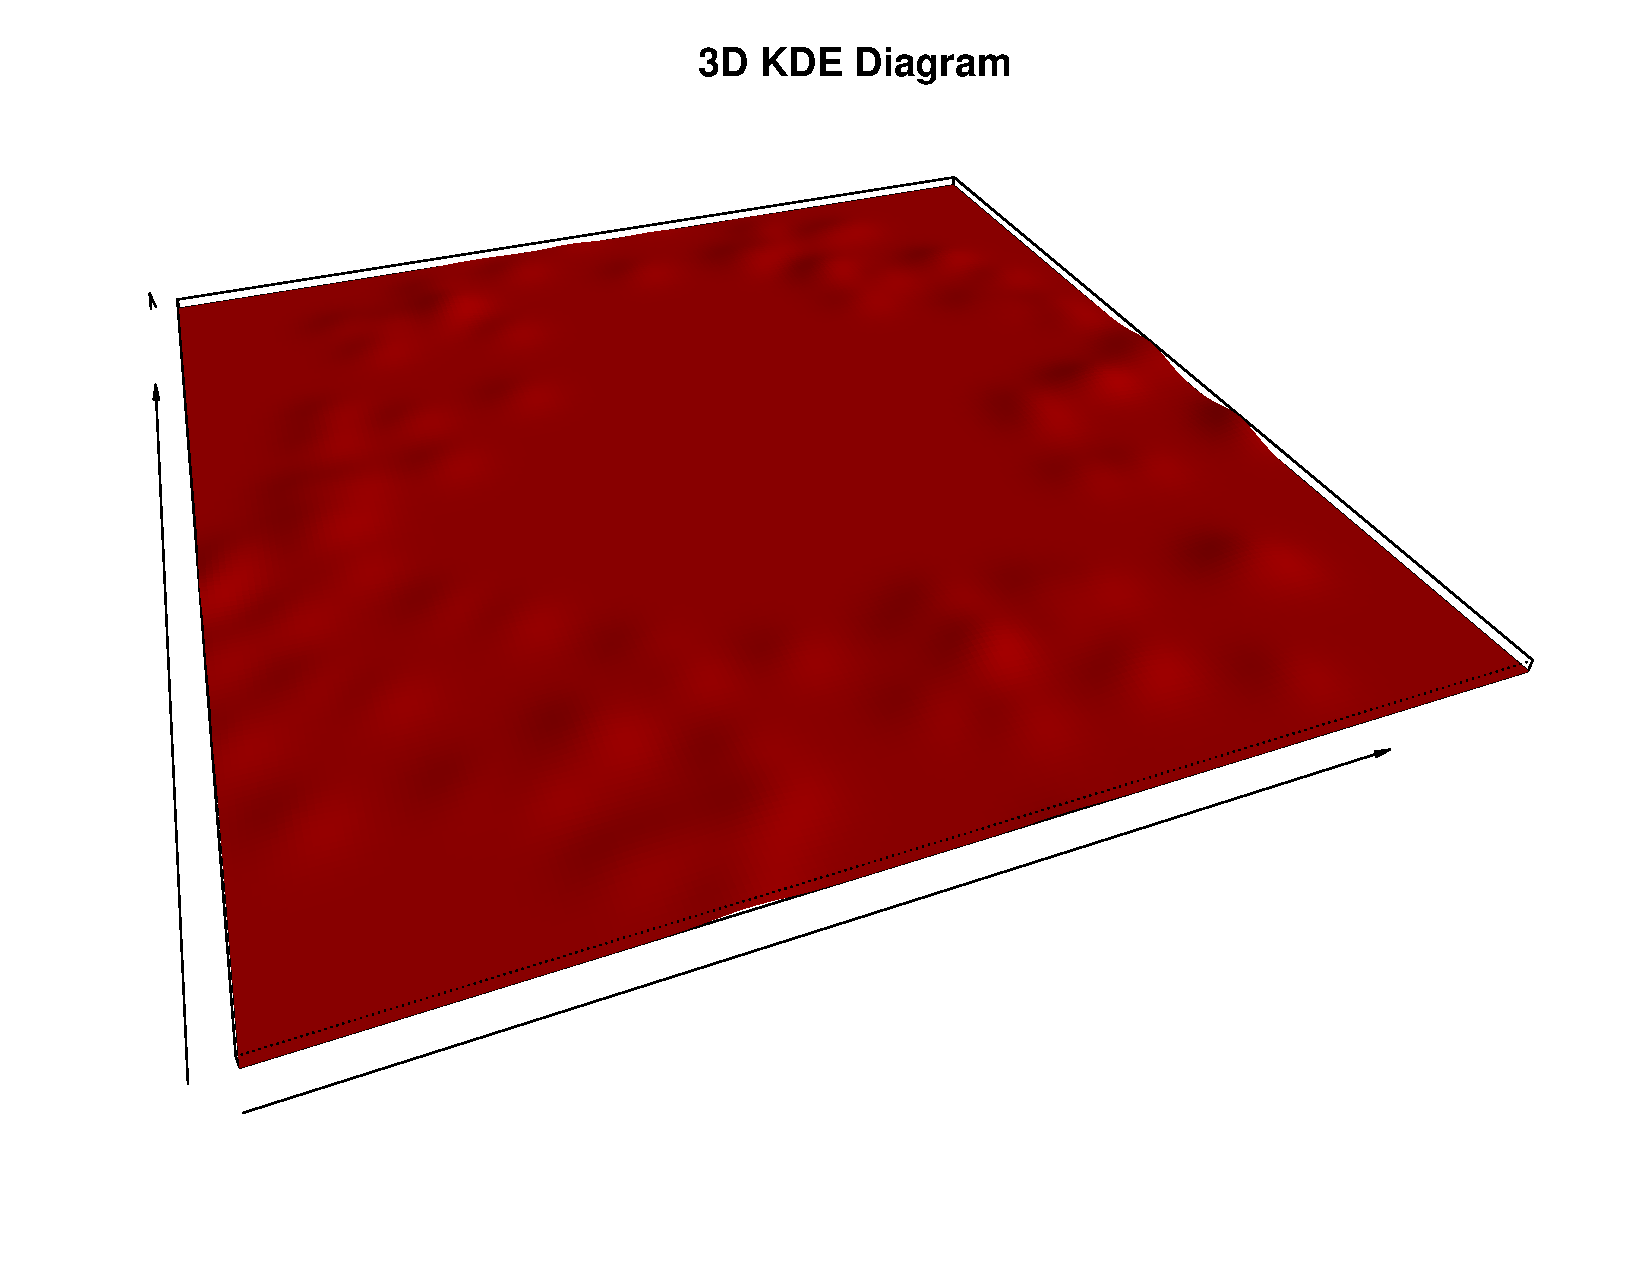
\includegraphics[width=\linewidth]{noisycircle2}
\end{subfigure}%
\begin{subfigure}{.32\textwidth}
  \centering
  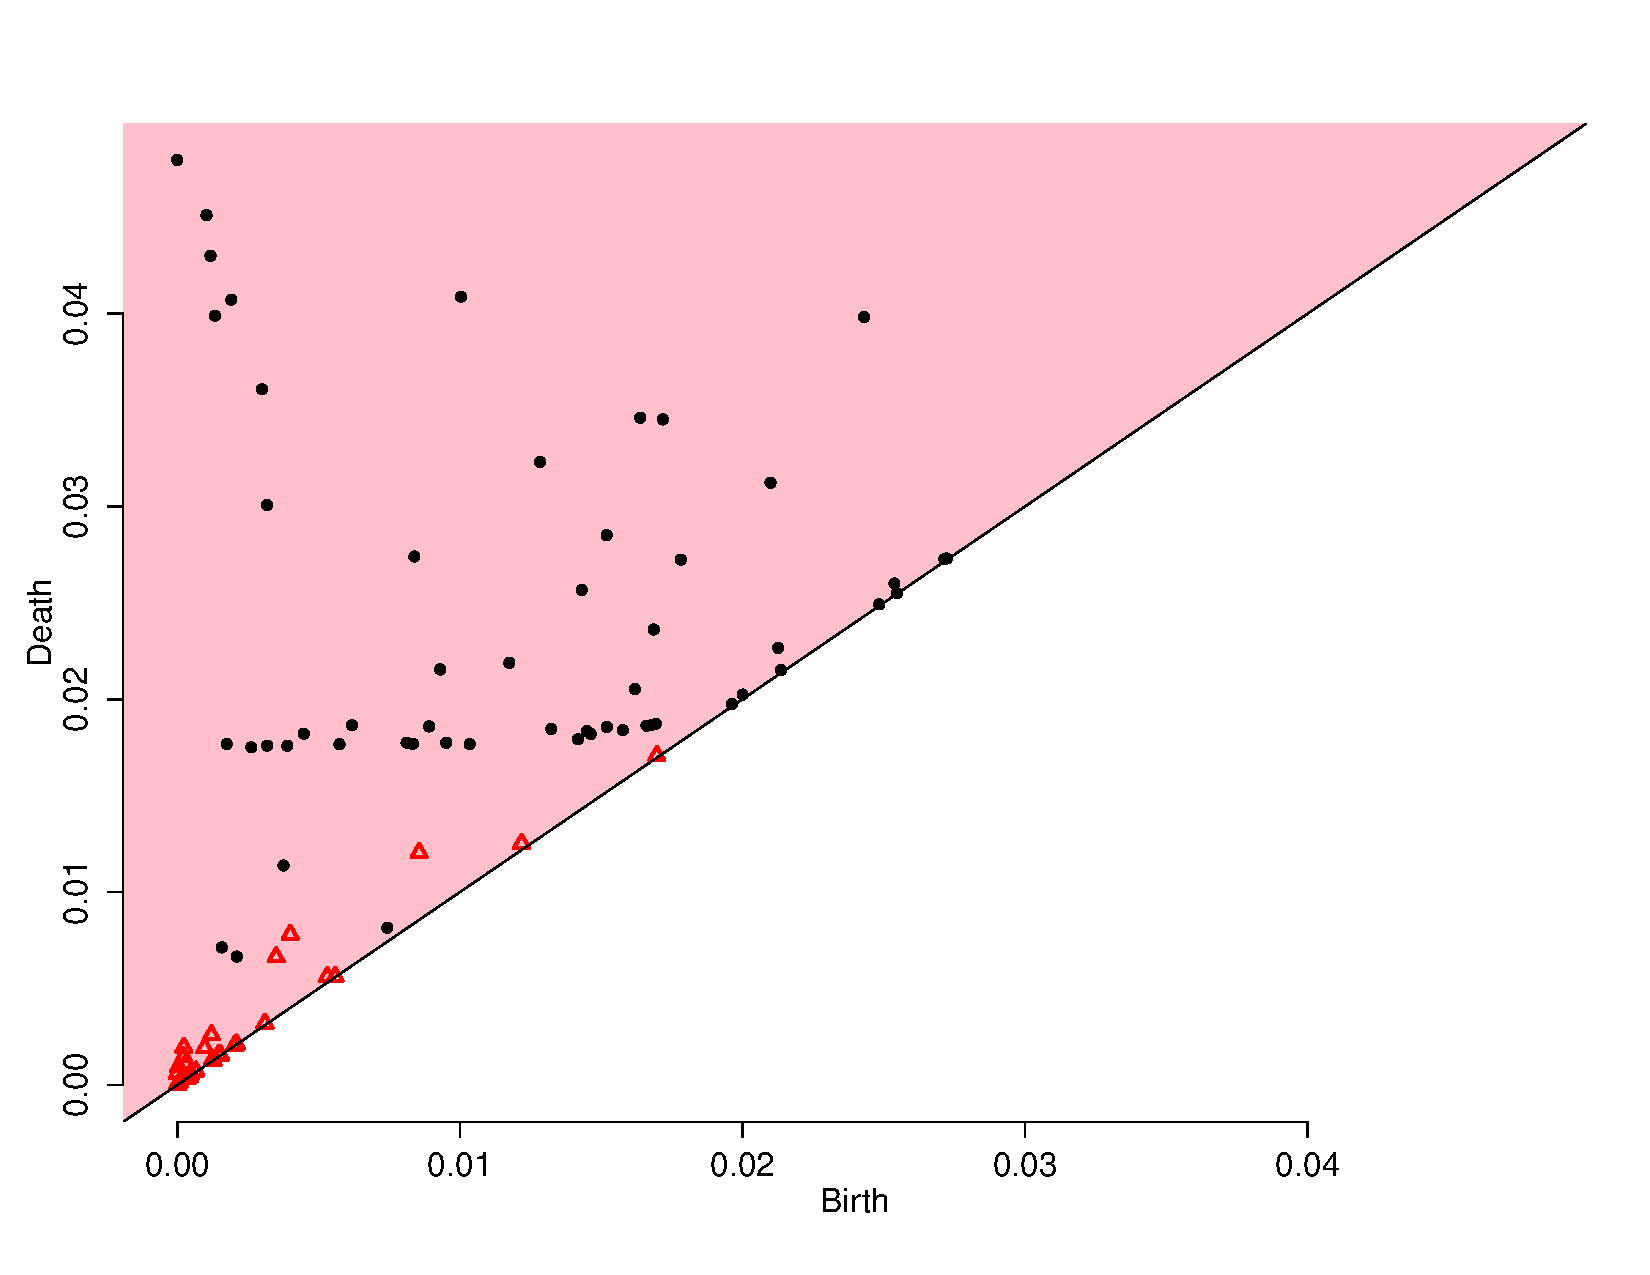
\includegraphics[width=\linewidth]{noisycircle3}
\end{subfigure}
\caption{(left) Noisy circle data. (middle) The topology of the perturbed circle. Notice the several clumps of local maxima. (right), A single persistence diagram. There are several shortlived 1st homology features, and only a couple persistent ones. There are several long-living 0th order homology features. }
\end{figure}

\subsection{Adding Additional Points}
Instead of perturbing the points themselves, additional gaussian samples are added around the circle. This should again, be an easier problem than the previous one. There still is a clear circular structure, albeit distractions all around. Looking at the data, the main loop was not found. All of the 1st order homology features had very short lives, indicating that could not have been the loop. And if they were, they must of immediately been distracted by the noise. From these observations, I think that Kernel Density Estimate also does not do well with noise. In general, I think topological methods are not good at handling noise. Intuitively it is hard to not consider a point if you do not know the final object's shape. Then, it's possible to find objects that are not actually there. \textbf{The only solution is to rerun the simulations over and over and look for significant objects.} But even then, I am not sure if the object that appears is noise or significant. 

\begin{figure}[htp!]
\centering
\begin{subfigure}{.32\textwidth}
  \centering
  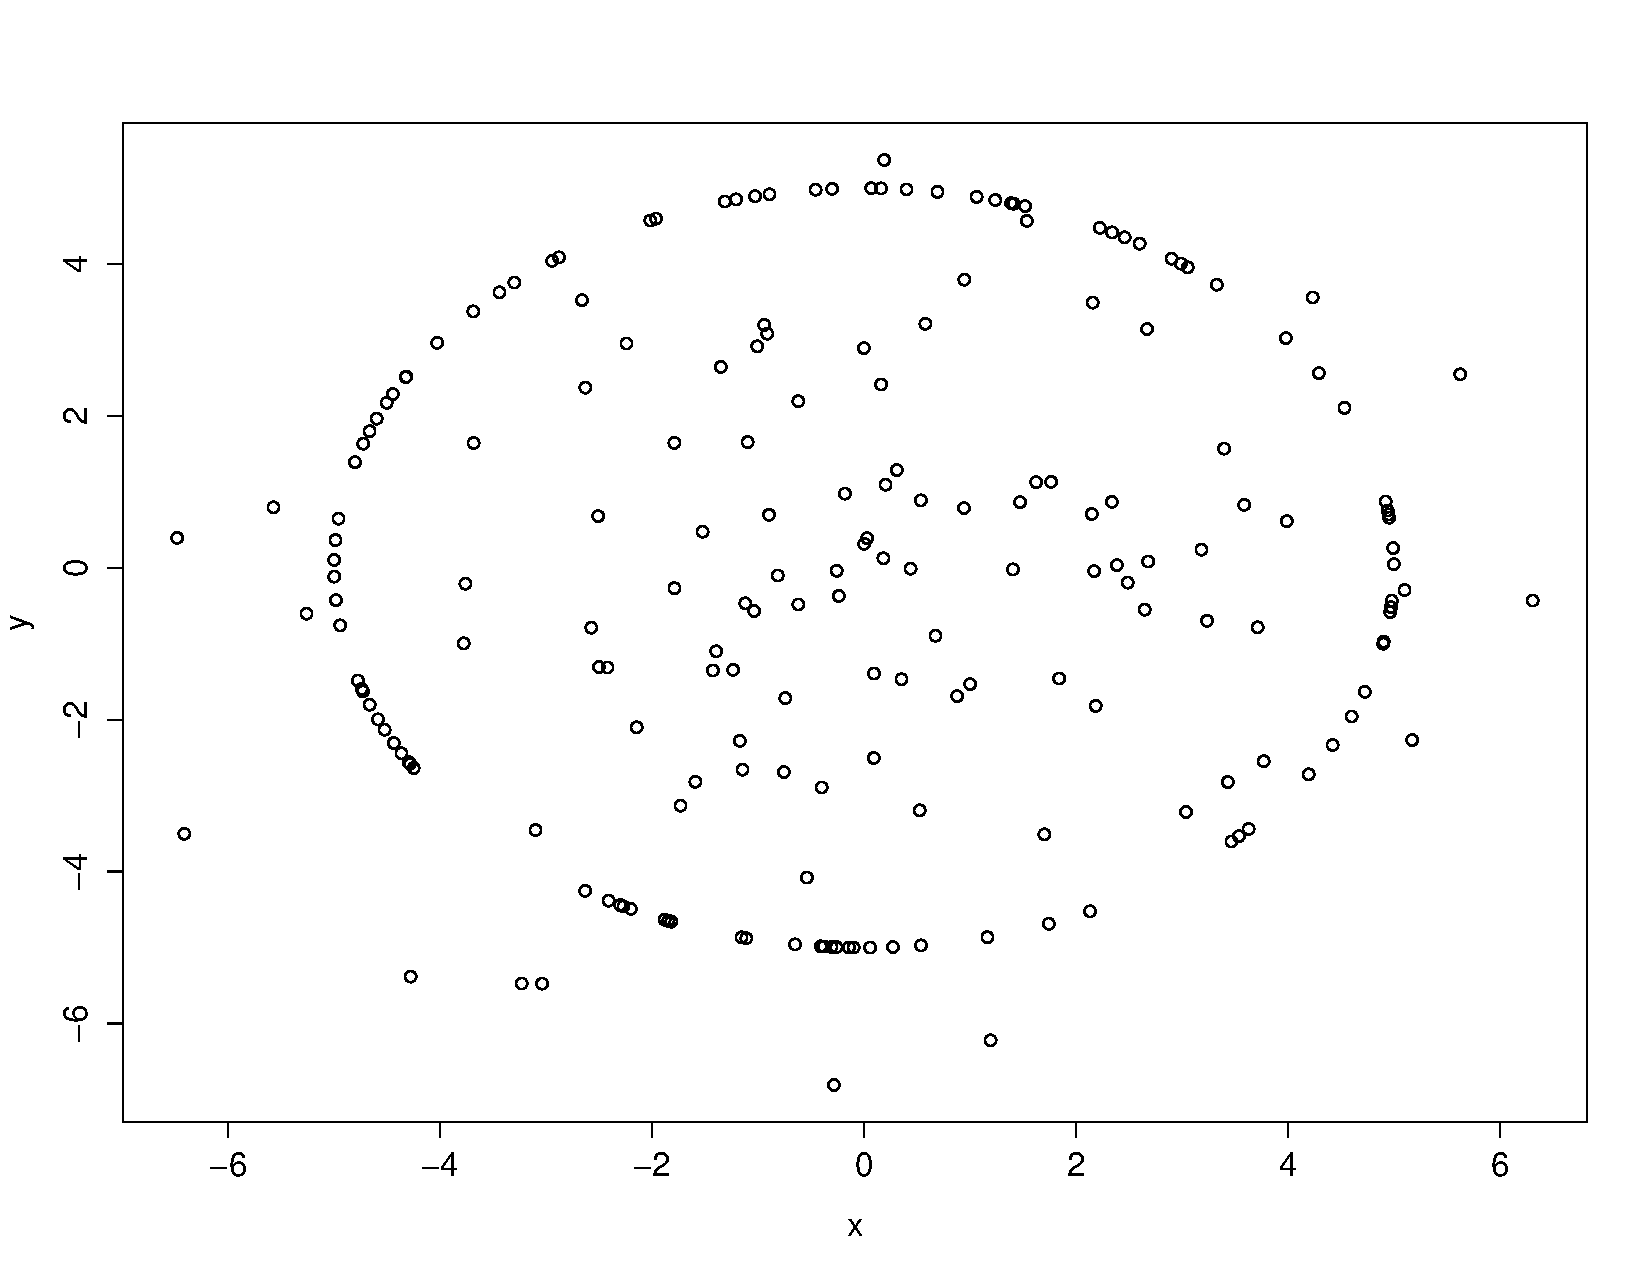
\includegraphics[width=\linewidth]{noisycircle1b}
\end{subfigure}%
\begin{subfigure}{.32\textwidth}
  \centering
  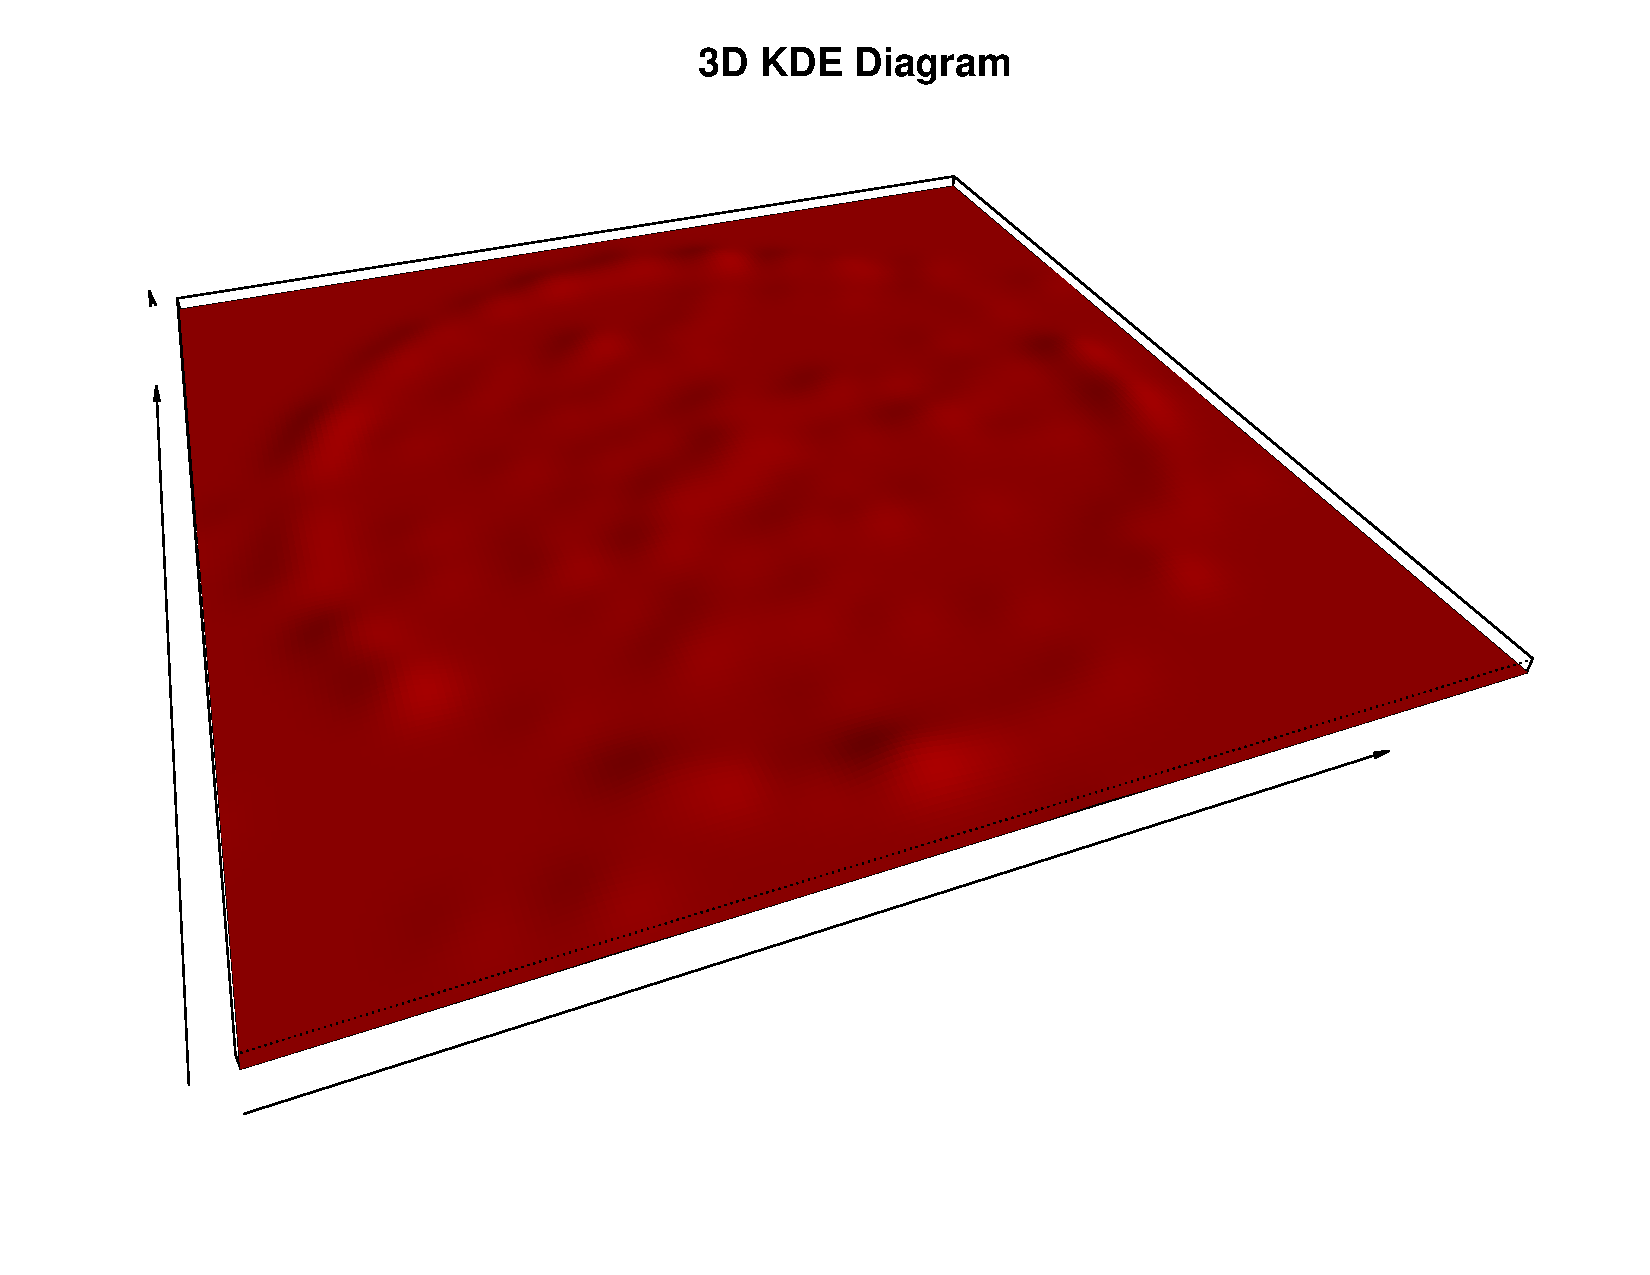
\includegraphics[width=\linewidth]{noisycircle3b}
\end{subfigure}%
\begin{subfigure}{.32\textwidth}
  \centering
  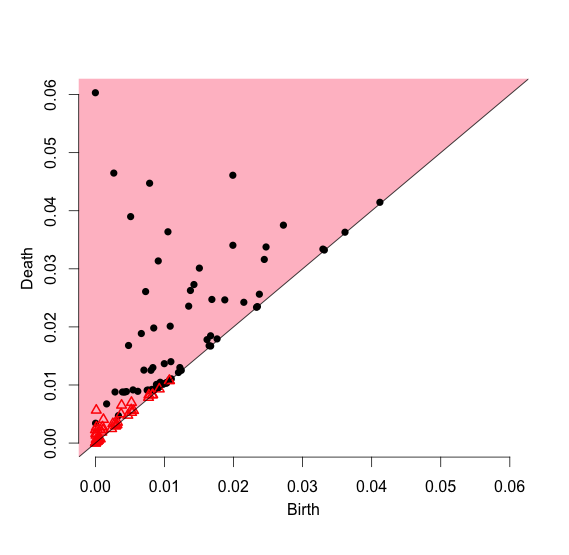
\includegraphics[width=\linewidth]{noisycircle2b}
\end{subfigure}
\caption{(left) Noisy circle data. (middle) The topology of the circle w/ extra points. Notice the several clumps of local maxima, esp in the middle. (right), A single persistence diagram. There are several shortlived 1st homology features,  and several long-living 0th order homology features. }
\end{figure}

\section{Persistence Diagrams on Hypothesis Testing}

\end{document}